% Licencia y derechos: consulte ../../LICENSE-CC-BY-4.0.
% Las figuras y demás materiales de terceros pueden tener derechos separados y deben identificarse.

\chapter{Estabilidad y osciladores} %p183
\section{Introducción} %p183
Un oscilador es un sistema que genera una señal periódica. Esquemáticamente se representa en la Figura \ref{fig:osc_basic}.

\begin{figure}[h]
	\centering
	\includegraphics[width=0.7\linewidth]{_fig/osc_basic.pdf}
	\caption{Un oscilador}
	\label{fig:osc_basic}
\end{figure}

Se distingue entre los generadores de onda sinusoidal, y los generadores de onda cuadrada o rectangular. Generalmente, los osciladores generadores de onda sinusoidal se implementan en dispositivos electrónicos trabajando de forma lineal, mientras los generadores de onda cuadrada o rectangular trabajan los dispositivos en forma no-lineal. Por ahora, nos interesa los osciladores que generan ondas sinusoidales, es decir, estaremos trabajando con dispositivos que trabajan en forma lineal. La discusión de generadores de onda cuadrada o rectangular tiene un enfoque notablemente distinto.

El esquema de la Figura \ref{fig:osc_basic} se ha omitido la fuente de polarización que energiza el sistema. En la Figura  \ref{fig:osc_basic-dc} se indica esta fuente de DC. Esta figura destaca otra interpretación del oscilador, que es de un convertidor de corriente continua a corriente alterna. En cualquier caso, el oscilador es un sistema no-lineal, bien esta porque genera una frecuencia de salida que no es suministrada por la entrada (la fuente DC), o porque la genera sin tener entrada (la fuente DC sólo polariza el circuito). Se podría considerar como un sistema marginalmente estable, ya que la amplitud de la señal no aumenta ni disminuye con el tiempo.

\begin{figure}[h]
	\centering
	\includegraphics[width=0.7\linewidth]{_fig/osc_basic-dc.pdf}
	\caption{Un oscilador, polarizado con una fuente DC}
	\label{fig:osc_basic-dc}
\end{figure}

Un sistema que genera una señal sinusoidal es marginalmente estable y tiene sus polos sobre el eje imaginario; su función de transferencia podría ser de la siguiente forma:

\( H(s) = \frac{a}{s^2 + a^2} \), con polos en \( s^2 = -a^2 \), es decir, \( s = \pm ja \)

Tal como se indica en la Figura \ref{fig:osc_sine_polos-y-ceros}, la frecuencia de oscilación es \( a \).

\begin{figure}[h]
	\centering
	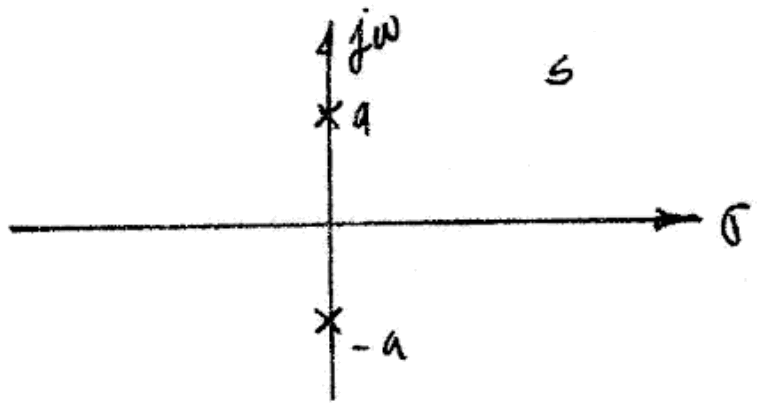
\includegraphics[width=0.7\linewidth]{_fig/osc_sine_polos-y-ceros.png}
	\caption{Diagrama de polos y ceros de onda sinusoidal}
	\label{fig:osc_sine_polos-y-ceros}
\end{figure}

Hay ocasiones cuando queremos un circuito que oscile a una determinada frecuencia. Pero también hay la posibilidad que un circuito oscile cuando no deseamos ese comportamiento; por ejemplo, hay configuraciones de amplificadores de alta ganancia que "estallan" en oscilaciones permanentes.

Estos dos casos están relacionados. En este tema vamos a querer aprender lo siguiente: ¿Por qué oscila un circuito? ¿Cómo evitar que un circuito oscile cuando no lo deseamos? ¿Cómo diseñar un circuito para que oscile a una determinada frecuencia?

\subsection{Ejemplo}
\begin{figure}[h]
	\centering
	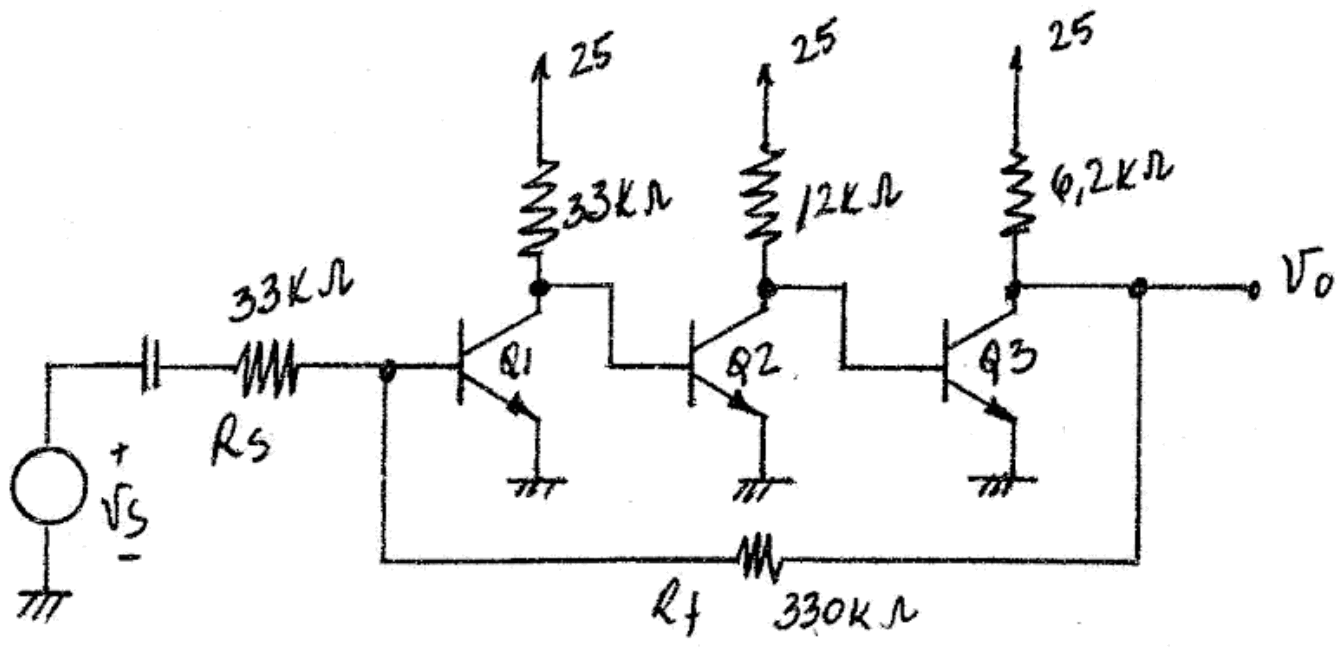
\includegraphics[width=0.7\linewidth]{_fig/osc_ejm1.png}
	\caption{Circuito de tres etapas con retroalimentación}
	\label{fig:osc_ejm1}
\end{figure}

Uno de los circuitos que se vio en el tema de retroalimentación fue la configuración de tres etapas con muestreo de nodo - comparación de nodo que se muestra en la Figura \ref{fig:osc_ejm1}. En principio, es una configuración de retroalimentación negativa. Sin embargo, se montó en el laboratorio y empezó a oscilar. ¿Qué pasó?

\begin{figure}[h]
	\centering
	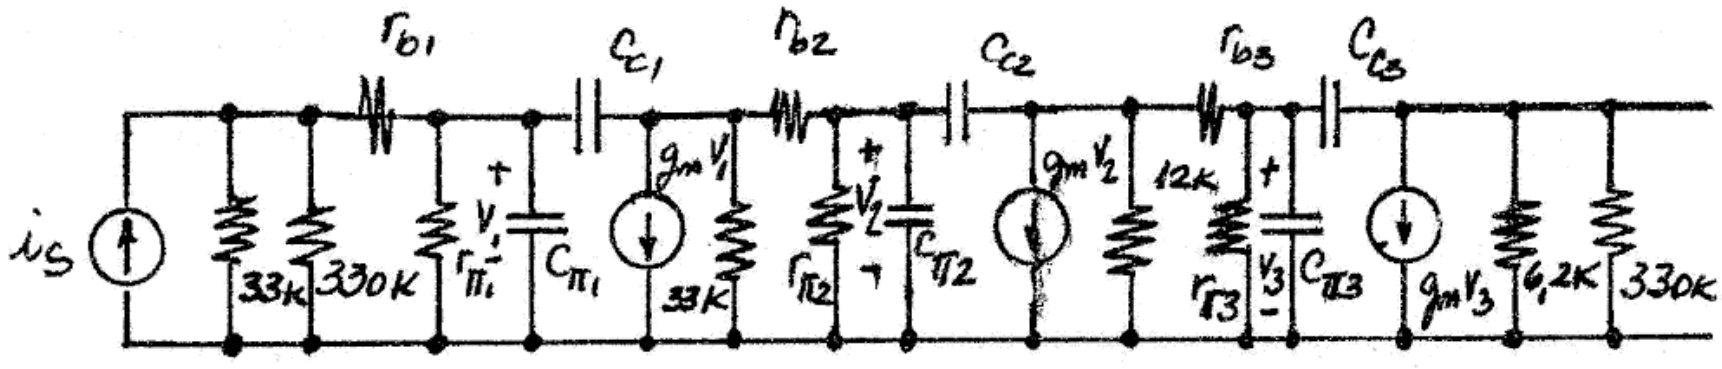
\includegraphics[width=0.7\linewidth]{_fig/osc_ejm1_alta-frecuencia.png}
	\caption{Modelo de alta frecuencia de la Figura \ref{fig:osc_ejm1}}
	\label{fig:osc_ejm1_alta-frecuencia}
\end{figure}

Recordemos que la retroalimentación negativa exige que \( A \) y \( B \) tengan el mismo signo \( - \) y en efecto, a frecuencias medias, el circuito de arriba cumple con esta condición. Sin embargo, al considerar la ganancia del amplificador sin retroalimentación, y el modelo de alta frecuencia del transistor, como se muestra en la Figura \ref{fig:osc_ejm1_alta-frecuencia}, el circuito presenta polos de alta frecuencia. En una aproximación de primer orden, se asocia un polo dominante por cada transistor, de modo que el circuito tiene tres polos. Cada polo introduce un desfase que es de \( 0^\circ \) a frecuencias bajas y medias, y llega a un valor mínimo de \( -90^\circ \). Por lo tanto, si se consideran los tres polos, van a cambiar el desfase inicial de \( A \) por la cantidad de \( -270^\circ \); en particular, lo llegan a cambiar por \( -180^\circ \), lo que representa un cambio de signo. 

Por lo tanto, si a frecuencias medias \( A \) y \( \beta \) son del mismo signo, a otra frecuencia superior serán de signo opuesto, y el sistema que cumple con las condiciones de retroalimentación negativa a frecuencias medias, se convierte en un sistema de retroalimentación positiva, provocando una inestabilidad que puede manifestarse en la forma de oscilaciones.

En este tema queremos estudiar esta condición de oscilación, bien sea para evitarla, tal vez con una compensación de frecuencia, o para buscarla y así crear el tipo de circuito conocido como oscilador.

Una técnica gráfica que indica el comportamiento oscilatorio de un sistema al ser sometido a retroalimentación es \textbf{el lugar geométrico de las raíces}. En principio, la función de transferencia del amplificador viene dada por \( A(s) \). Al someter el amplificador a una retroalimentación \( \beta \), surge la función de transferencia del amplificador con retroalimentación:

\begin{equation}
	A_f(s) = \frac{A(s)}{1 + A(s)\beta}
\end{equation}

Evidentemente, las raíces del sistema cambiarán; además, su ubicación será función del valor de \( \beta \). Por lo tanto, la técnica del lugar geométrico de las raíces describe la trayectoria de las raíces del sistema a medida que \( \beta \) aumenta.

Consideramos tres casos por ahora:
sistemas sin retroalimentación de un polo real y negativo,
dos polos reales y negativos,
y tres polos reales y negativos 

\begin{figure}[h]
	\centering
	\subfloat[1 polo]
	{
		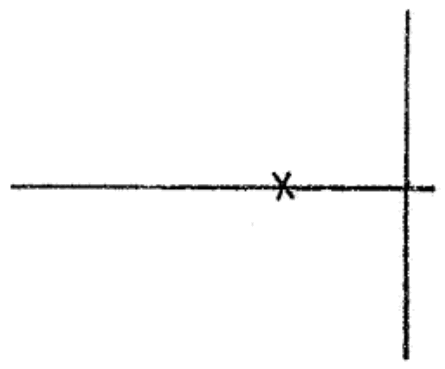
\includegraphics[width=0.3\linewidth]{_fig/osc_3roots-1.png}
		\label{fig:osc_3roots-1}
	}
	\subfloat[2 polos]
	{
		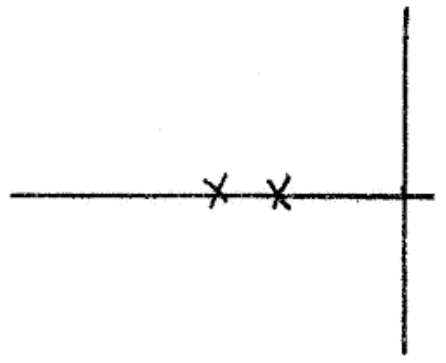
\includegraphics[width=0.3\linewidth]{_fig/osc_3roots-2.png}
		\label{fig:osc_3roots-2}
	}
	\subfloat[3 polos]
	{
		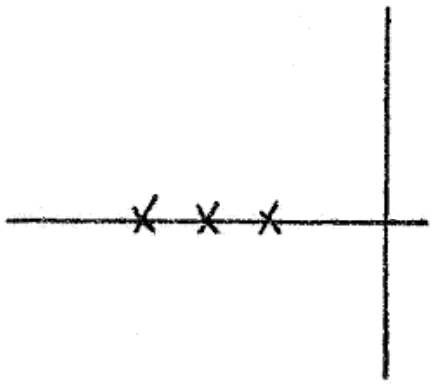
\includegraphics[width=0.3\linewidth]{_fig/osc_3roots-3.png}
		\label{fig:osc_3roots-3}
	}
	\caption{Lugar geométrico de raíces de 3 sistemas}
	\label{fig:osc_3roots}
\end{figure}

\begin{figure}[h]
	\centering
	\subfloat[1 polo]
	{
		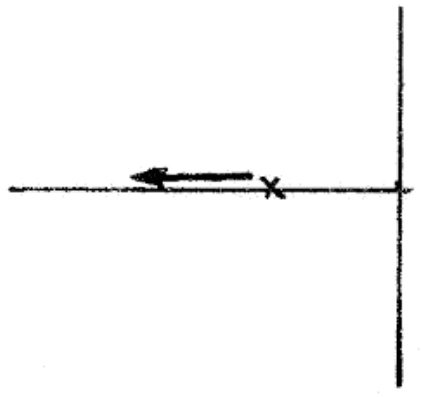
\includegraphics[width=0.3\linewidth]{_fig/osc_3roots-1-wt.png}
		\label{fig:osc_3roots-1-wt}
	}
	\subfloat[2 polos]
	{
		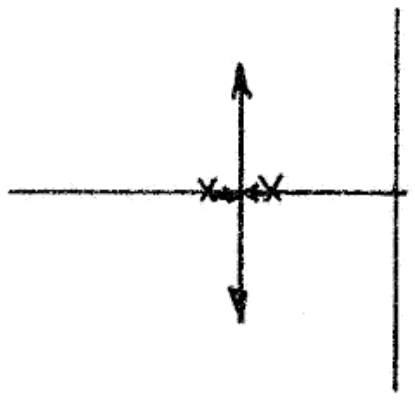
\includegraphics[width=0.3\linewidth]{_fig/osc_3roots-2-wt.png}
		\label{fig:osc_3roots-2-wt}
	}
	\subfloat[3 polos]
	{
		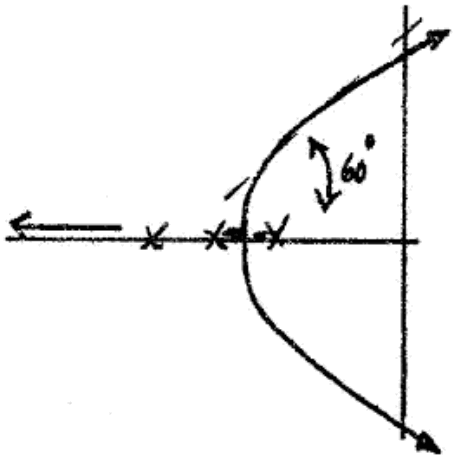
\includegraphics[width=0.3\linewidth]{_fig/osc_3roots-3-wt.png}
		\label{fig:osc_3roots-3-wt}
	}
	\caption{Lugar geométrico de raíces de 3 sistemas, con trazas}
	\label{fig:osc_3roots-wt}
\end{figure}

Se muestran en las Figuras \ref{fig:osc_3roots-1}, \ref{fig:osc_3roots-2} y \ref{fig:osc_3roots-3}. En las Figuras \ref{fig:osc_3roots-1-wt}, \ref{fig:osc_3roots-2-wt} y \ref{fig:osc_3roots-3-wt} respectivamente, se traza la trayectoria de las raíces a medida que aumenta \( \beta \).

En el sistema de un solo polo, la Figura \ref{fig:osc_3roots-1}, a medida que aumenta \( \beta \), este polo se desplaza hacia la izquierda por el mismo eje real, la Figura \ref{fig:osc_3roots-1-wt}. Esto quiere decir que cuanto más retroalimentación tiene el sistema, mayor es su ancho de banda.

En base a funciones de transferencia, tenemos la del sistema sin retroalimentación:

\begin{equation}
	A(s) = \frac{A_0}{1 + j\frac{f}{f_H}}
\end{equation}

Con la cual se obtiene la del sistema con retroalimentación:

\begin{equation}
	A_f(s) = \frac{A_0}{1 + \beta A_0 + j\frac{f}{f_H}}
\end{equation}

De donde concluimos que la frecuencia de corte con retroalimentación en función de la frecuencia de corte sin retroalimentación viene dada por:

\begin{equation}
	f_{H\beta} = f_H (1 + A_0\beta)
\end{equation}

Lo cual demuestra lo dicho relativo al ancho de banda, se hace notar que la retroalimentación no modifica el producto ganancia-ancho de banda del sistema: en la medida que disminuye la ganancia, así mismo aumenta el ancho de banda.

En el sistema de dos polos, la Figura \ref{fig:osc_3roots-2}, a medida que aumenta \( \beta \), estos polos primero se acercan por el mismo eje real, y al encontrarse, se despegan del eje real en forma perpendicular a él, con una parte real constante y una parte imaginaria crecientemente más grande, la Figura \ref{fig:osc_3roots-2-wt}. Cuando la parte imaginaria supera en valor absoluto a la parte real, la respuesta de frecuencia tiene una resonancia que se hace más pronunciada a medida que aumenta la parte imaginaria, es decir, a medida que aumenta \( \beta \). Sin embargo, los polos permanecen en el plano izquierdo y el sistema es siempre estable.

Si la función de transferencia del sistema sin retroalimentación se expresa como:

\begin{equation}
	A(s) = \frac{A_0}{(1 + s/w_1)(1 + s/w_2)}
\end{equation}

Entonces la función de transferencia del sistema con retroalimentación viene dada por:

\begin{equation}
	A_f(s) = \frac{A_0 w_1 w_2}{s^2 + (w_1 + w_2)s + w_1 w_2 (1 + \beta A_0)}
\end{equation}

\begin{figure}[h]
	\centering
	\subfloat[Respuesta de frecuencia]
	{
		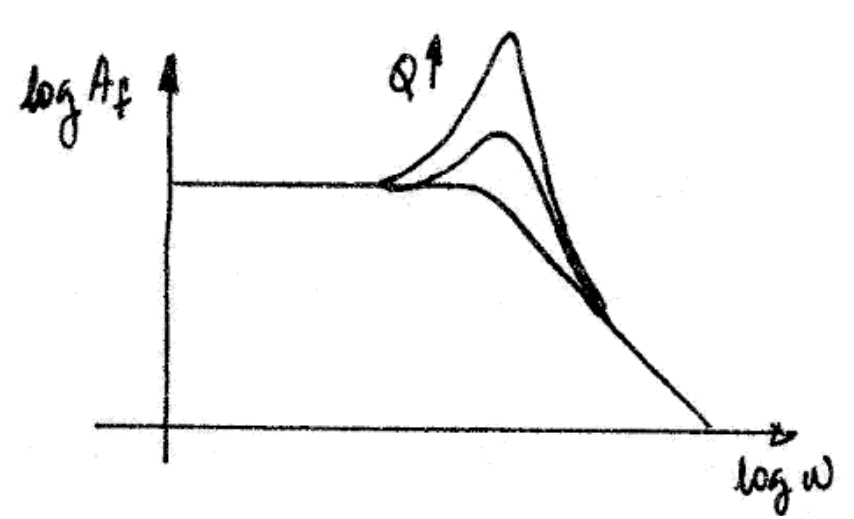
\includegraphics[width=0.45\linewidth]{_fig/osc_sys-2-polos-freq.png}
		\label{fig:osc_sys-2-polos-frec}
	}
	\subfloat[Respuesta a un escalón]
	{
		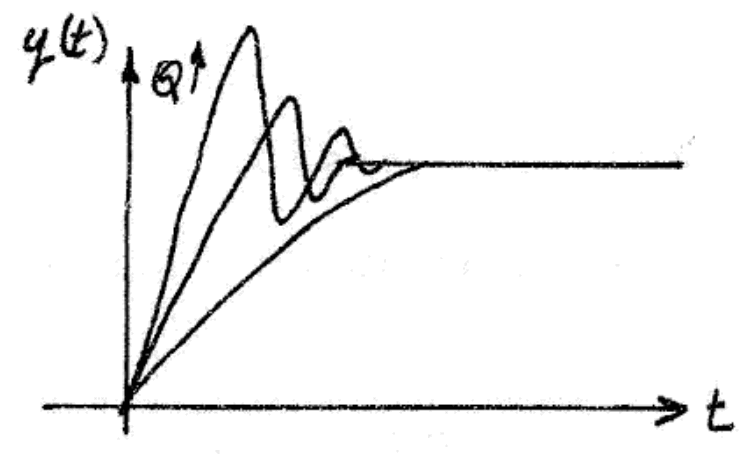
\includegraphics[width=0.45\linewidth]{_fig/osc_sys-2-polos-step.png}
		\label{fig:osc_sys-2-polos-step}
	}
	\caption{Sistema de dos polos}
	\label{fig:osc_sys-2-polos}
\end{figure}

En la Figura \ref{fig:osc_sys-2-polos} se muestra la respuesta de frecuencia y la respuesta a un escalón de sistemas de segundo orden en función de la calidad, \( Q \), del sistema.

En un sistema de tres polos, la Figura \ref{fig:osc_3roots-3}, a medida que aumenta la retroalimentación, el polo a la izquierda se va alejando del origen por el mismo eje real, y los dos polos más cerca al origen se acercan y se despegan con una trayectoria que se aproximan a asíntotas que hacen ángulos de \( \pm 60^\circ \) con el eje real, la Figura \ref{fig:osc_3roots-3-wt}. Con estas trayectorias se destaca que dado suficiente retroalimentación, los polos cruzan el eje imaginario y pasan al plano derecho. Entonces el sistema, que era estable en principio, puede convertirse en un sistema inestable dada suficiente retroalimentación. Dada la función de transferencia del sistema sin retroalimentación:

\begin{equation}
	A(s) = \frac{A_0}{(1 + s/w_1)(1 + s/w_2)(1 + s/w_3)}
\end{equation}

La función del sistema con retroalimentación puede expresarse como:

\begin{equation}
	A_f(s) = \frac{A_0}{\left[ \left(\frac{s}{w_0}\right)^3 + a_2 \left(\frac{s}{w_0}\right)^2 + a_1 \left(\frac{s}{w_0}\right) + 1 \right]}
\end{equation}

Finalmente, otro enfoque para entender las condiciones de oscilación analiza la expresión de la ganancia con retroalimentación:

\begin{equation}
	A_f = \frac{A}{1 + A\beta}
\end{equation}

Evidentemente, si \( A\beta = -1 \), la ganancia tiende a \( \infty \) y el sistema es inestable. La relación \( A\beta = -1 \), o también \( -A\beta = 1 \), es conocida como el criterio de \textbf{Barkhausen} para que un sistema oscile. La expresión \( -A \beta \) es la \textbf{ganancia de lazo} que presentamos en el tema anterior y representa la relación entre una señal aplicada en cualquier punto del lazo, y la señal que regresa a ese punto alrededor del lazo. Si esta ganancia es igual a uno con cero desfasaje tenemos un oscilador. Ver la Figura \ref{fig:osc_ganancia-lazo}.

\begin{figure}[h]
	\centering
	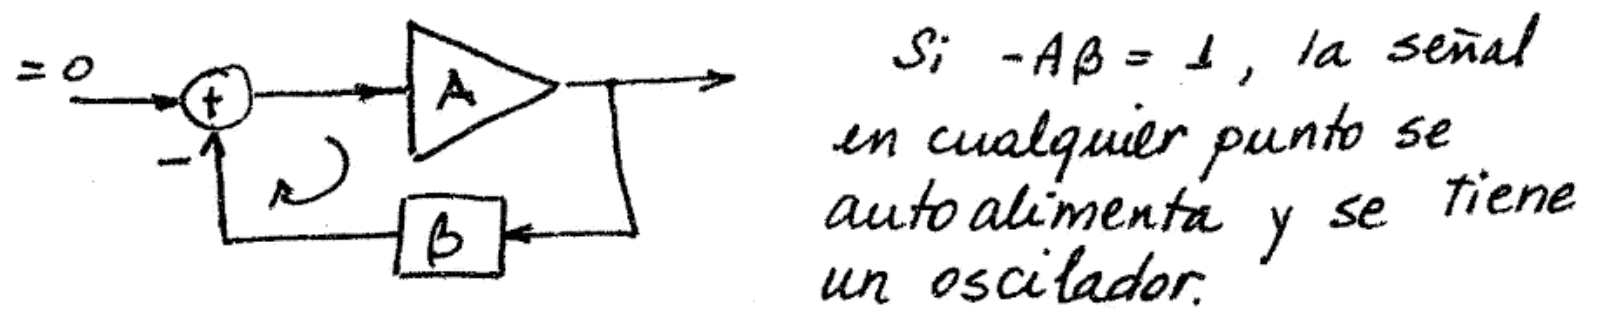
\includegraphics[width=0.8\linewidth]{_fig/osc_ganancia-lazo.png}
	\caption{Ganancia del lazo \( = -A \beta \)}
	\label{fig:osc_ganancia-lazo}
\end{figure}

\section{Estabilidad} %190

Hemos visto que existe el riesgo de oscilación al introducir retroalimentación en amplificadores conformados con al menos 3 etapas. En el diseño de amplificadores es necesario asegurar que el circuito sea estable a todas las frecuencias, y no limitarse a cierto rango de interés.

Esto exige que los polos de la función de transferencia, es decir, los ceros de \( 1 + A\beta \) se encuentren en el plano izquierdo. Hay otros criterios que también permiten determinar la estabilidad de un sistema con retroalimentación.

\subsection{El criterio de Nyquist} %p190

Se grafica el número complejo \( A\beta \) en el plano complejo para \( f \) entre \( -\infty \) y \( +\infty \). Si la curva resultante encierra el punto \( -1+j0 \), el amplificador es inestable; si no lo encierra, entonces es estable.

\textbf{Ejemplo:} Si tenemos un sistema de un solo polo:

\[
\beta A = \frac{\beta A_0}{(1+jf/f_H)} = \frac{\beta A_0 (1 - jf/f_H)}{1+(f/f_H)^2}
\]

Dejando que \( A_0 = 1000 \), \( f_H = 2000 \), \( \beta = 0.1 \), las expresiones para las partes real e imaginaria de \( \beta A \) son:

\[
\text{Re}|\beta A| = \frac{\beta A_0}{1 + (f/f_H)^2} = \frac{100}{1 + (f/2000)^2}
\]

\[
|\text{Im}[\beta A]| = \frac{-\beta A_0 f}{f_H [1+(f/f_y)^2]} = \frac{100f}{2000[1+(f/2000)^2]}
\]

Sustituyendo valores se obtienen los siguientes resultados; se hace notar que para $f$ negativo cambia el signo con respecto al resultado para $f$ positivo; se grafican en la Figura \ref{fig:osc_ab-plano-complejo}. La curva inferior es para $f$ positivo, y la superior, el imagen espejo de la inferior, es para $f$ negativo. Como "$-1$" no está en el interior (definido como a la izquierda \textit{cuando se va de $-\infty$ a $+\infty$}) de la forma, entonces es un sistema estable.

\begin{tabular}{c|cccccccccc}
	$f$     & 10  & 100 & 1000 & 2000 & 3000 & 4000 & 5000 & 10k  & 100k \\
	Re$[\beta A]$ & 100 & 99.7 & 88   & 50   & 30.7 & 20   & 13.8 & 3.85 & 0.04 \\
	Im$[\beta A]$ & -0.5& -4.9 & -40  & -50  & -46  & -40  & -34  & -19  & -2 \\
\end{tabular}

%			\begin{table}[H]
	%				\centering
	%				\caption*{Valores de $\text{Re}[\beta A]$ y $\text{Im}[\beta A]$ para $f>0$}
	%				\begin{tabular}{c|cccccccccc}
		%					$f$     & 10  & 100 & 1000 & 2000 & 3000 & 4000 & 5000 & 10k  & 100k \\
		%					\midrule
		%					Re$[\beta A]$ & 100 & 99.7 & 88   & 50   & 30.7 & 20   & 13.8 & 3.85 & 0.04 \\
		%					Im$[\beta A]$ & -0.5& -4.9 & -40  & -50  & -46  & -40  & -34  & -19  & -2 \\
		%				\end{tabular}
	%			\end{table}
%			
%			\begin{table}[H]
	%				\centering
	%				\caption*{Valores de $\text{Re}[\beta A]$ y $\text{Im}[\beta A]$ para $f<0$}
	%				\begin{tabular}{c|cccccccccc}
		%					$f$     & -10  & -100 & -1k  & -2k  & -3k  & -4k  & -5k  & -10k  & -100k \\
		%					\midrule
		%					Re$[\beta A]$ & 100  & 99.7 & 88   & 50   & 30.7 & 20   & 13.8 & 3.85  & 0.04 \\
		%					Im$[\beta A]$ & +0.5 & +4.9 & +40  & +50  & +46  & +40  & +34  & +19   & +2 \\
		%				\end{tabular}
	%			\end{table}

\begin{figure}[h]
	\centering
	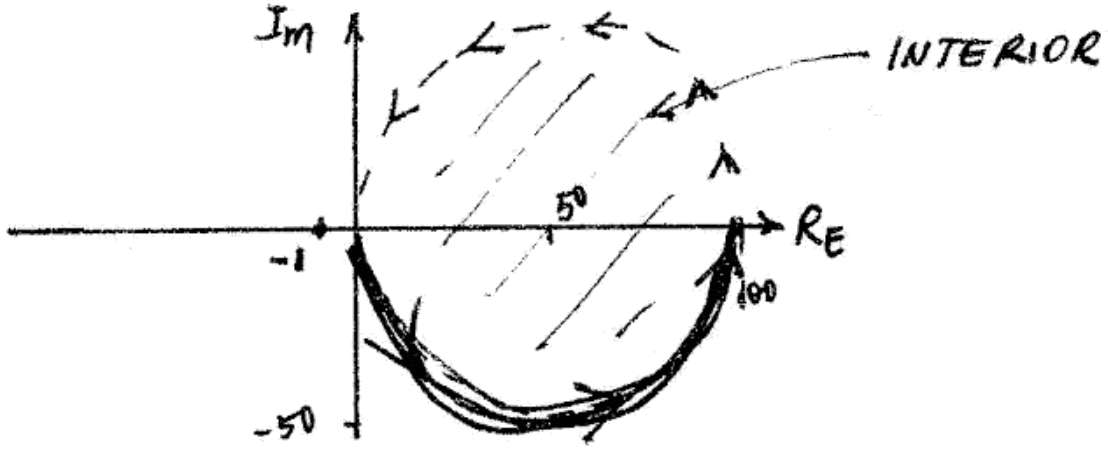
\includegraphics[width=0.8\linewidth]{_fig/osc_ab-plano-complejo.png}
	\caption{La gráfica de $A \beta$ en el plano complejo}
	\label{fig:osc_ab-plano-complejo}
\end{figure}

\subsection{Margen de Fase y de Ganancia}

Otro método útil para determinar la estabilidad de un circuito es el del \textbf{Margen de Fase y de Ganancia}. Es un método gráfico basado en el Diagrama de Bode del producto $A \beta$ que procura garantizar que su módulo sea menor que 1 cuando su desfase es de $180^\circ$, y/o que el desfase sea mayor de $-180^\circ$	cuando la ganancia es \(|1|\), en la Figura \ref{fig:osc_margen-ganancia-fase} se indica cómo puede medirse estos márgenes sobre el Diagrama de Bode de $A \beta$.

\begin{figure}[h]
	\centering
	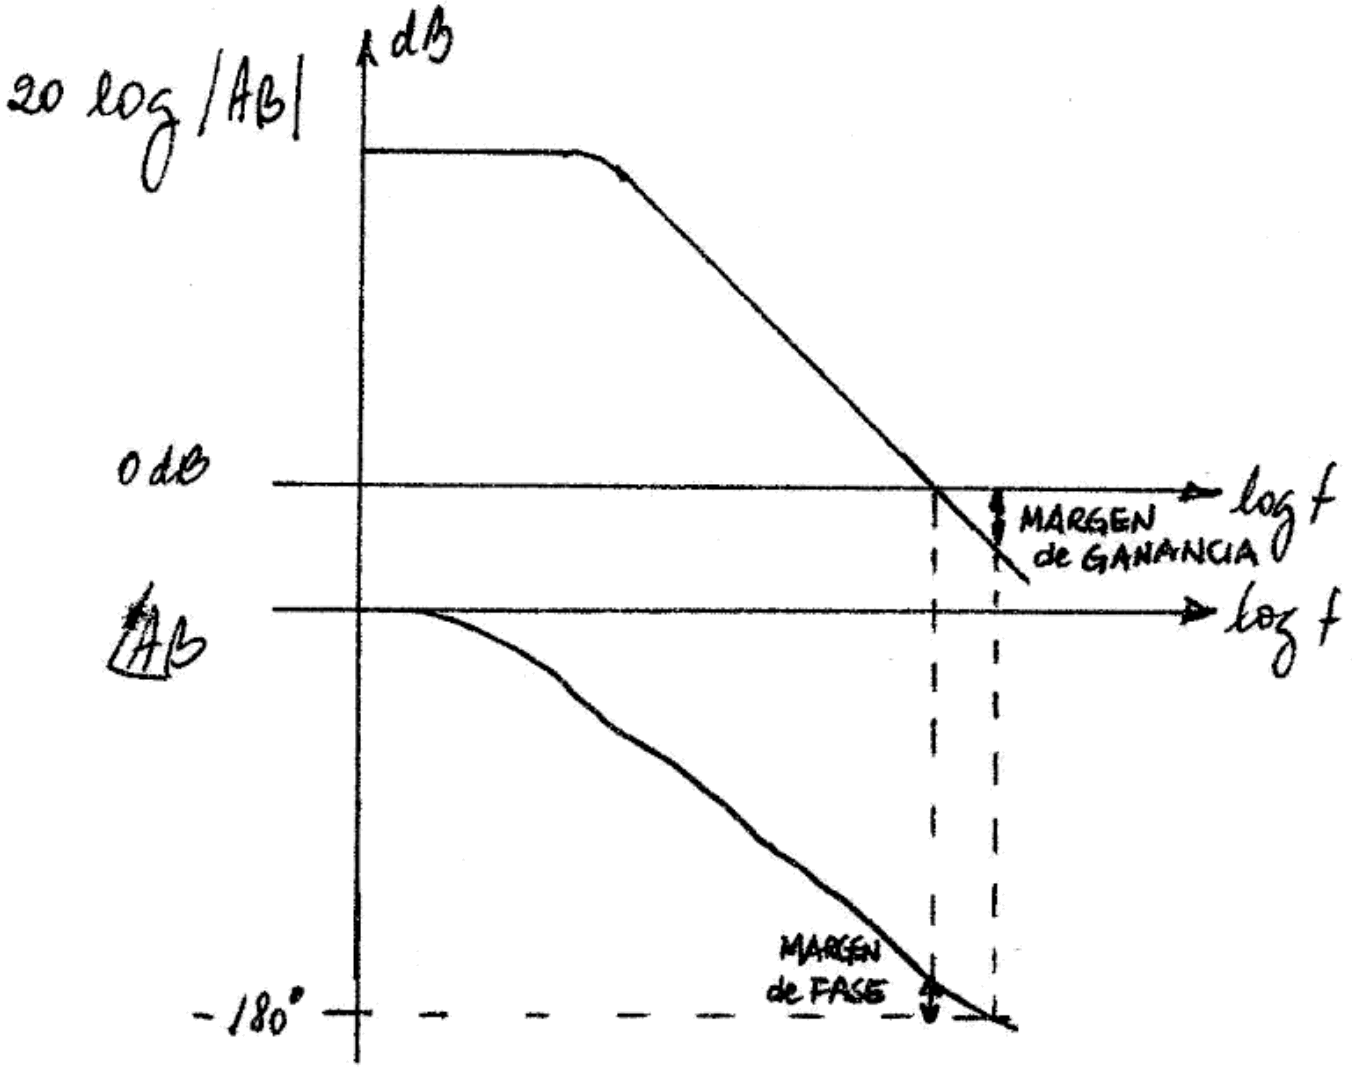
\includegraphics[width=0.8\linewidth]{_fig/osc_margen-ganancia-fase.png}
	\caption{Margen de Ganancia y de Fase}
	\label{fig:osc_margen-ganancia-fase}
\end{figure}

El \textbf{Margen de Ganancia} es la diferencia entre la ganancia a \( 180^\circ \) de fase y 0 dB; tiene que ser negativa para un sistema estable.

El \textbf{Margen de Fase} es la diferencia entre \( 180^\circ \) y la fase a 0 dB de ganancia; la fase a 0 dB de ganancia debería ser superior a \( -180^\circ \) por un margen de por lo menos \( 30^\circ \) para dar un sistema estable.

\subsubsection{Ejemplo 1}

Dado:

\[
A(s) = \frac{10000}{(1 + j f / 10^4)(1 + j f / 5 \times 10^4)(1 + j f / 10^5)}
\]

\begin{itemize}
	\item[a)] Determine la estabilidad del sistema con \( \beta = 0.1 \) por medio del criterio de Nyquist.
	\item[b)] Determine el Margen de Ganancia y de Fase.
\end{itemize}

\textbf{Solución:}

\textbf{a)} Determinación de la estabilidad del sistema con el criterio de Nyquist

La función \( A\beta \) se expresa como:

\[
A\beta = \frac{1000}{1 - 3.2 \times 10^{-7} f^2 + j f (1.3 \times 10^{-4} - f^2 / 5 \times 10^{13})}
\]

\[
A\beta = 1000 \frac{(1 - 3.2 \times 10^{-7} f^2) - j 1000 f (1.3 \times 10^{-4} - f^2 / 5 \times 10^{13})}{(1 - 3.2 \times 10^{-7} f^2)^2 + f^2 (1.3 \times 10^{-4} - f^2 / 5 \times 10^{13})^2}
\]

A partir de esta ecuación, se construyen las siguientes tablas:

\[
\begin{array}{|c|c|c|}
	\hline
	f & \text{Re} & \text{Im} \\
	\hline
	10 & 1000 & -1.3 \\
	100 & 999 & -13 \\
	1000 & 986 & -129 \\
	10k & 323 & -689 \\
	20k & -46 & -404 \\
	50k & -107 & -61 \\
	10^5 & -31 & 7 \\
	10^6 & -0.008 & 0.95 \\
	\hline
\end{array}
\]

\[
\begin{array}{|c|c|c|}
	\hline
	f & \text{Re} & \text{Im} \\
	\hline
	-10 & 1000 & +1.3 \\
	-100 & 999 & +13 \\
	-1k & 986 & +129 \\
	-10k & 323 & +689 \\
	-20k & -46 & +404 \\
	-50k & -107 & +61 \\
	-10^5 & -31 & -7 \\
	-10^6 & -0.008 & -0.95 \\
	\hline
\end{array}
\]

y en la Figura \ref{fig:osc_ejemplo1-nyquist} la gráfica correspondiente.

\begin{figure}[h]
	\centering
	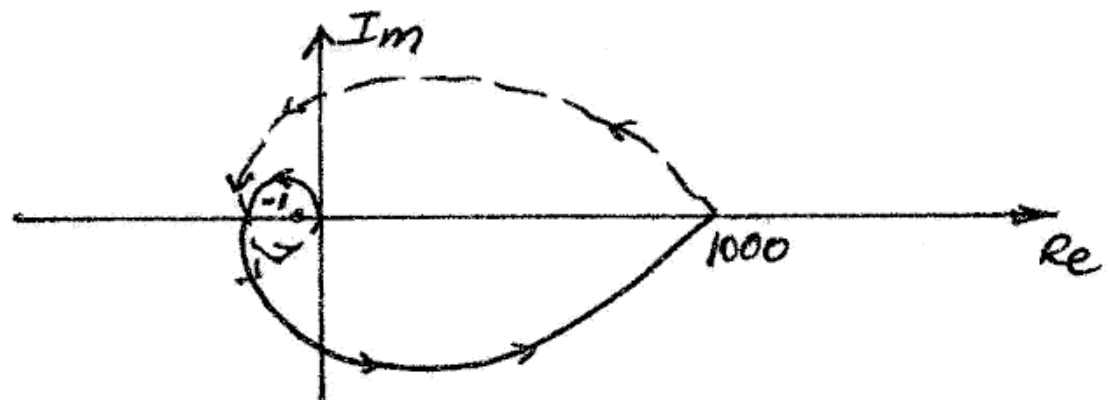
\includegraphics[width=0.8\linewidth]{_fig/osc_ejemplo1-nyquist.png}
	\caption{El criterio de Nyquist aplicado al Ejemplo 1}
	\label{fig:osc_ejemplo1-nyquist}
\end{figure}

La trayectoria de \( A\beta \) en el plano complejo, a medida que \( f \) varía de \( -\infty \) a \( +\infty \), encierra el punto \((-1,0)\), es decir, lo deja a su izquierda. Por lo tanto, concluimos que el sistema es \textbf{inestable} y tiende a oscilar.

\textbf{b)} Determinación del Margen de Ganancia y de Fase

Siguiendo con el problema anterior en su segunda parte, se espera llegar a la misma conclusión de que el sistema es inestable. El método es gráfico y orienta más a uno en cuanto a o que hace falta para convertir el sistema en uno estable.

En la Figura 4.11 se traza el diagrama de Bode aproximado de \( A\beta \); mostrando \( 20\log|A\beta| \) y la fase de \( A\beta \). Los puntos destacados incluyen las frecuencias de quiebre en \( f = 10^4 \), \( 5 \times 10^4 \) y \( 10^5 \), y la fase de \( A\beta \) ( \( \beta \) siendo real y positiva no midifica la fase de \( A \) ). Para determinar el margen de ganancia, buscamos la frecuencia a la cual el desfasaje es de \( -180\circ \) \( - \) aproximadamente en \( f = 75 \text{kHz} \), y a esa frecuencia \( 20\log|A\beta| \approx 36 \text{dB} \) (positivo!), es decir corresponde a un valor inestable. Para determinarl el Margen de Fase, buscamos la frecuencia a la cual al ganancia es \( 1 \) ( \( 0 \text{dB} \)): esto nos da \( f = 310 \text{kHz} \), para la cual el desfasaje es \( \approx -245 \circ < -180 \), es decir, nuevamente corresponde a un valor inestable. Una regla muy sencilla de aplicar para determinar si un sistema es inestable es la siguiente:

Si \( f_{0\text{dB}} = f_{180\circ} \) entonces el sistema es inestable: en la Figura \ref{fig:osc_ejemplo1-bode}, \( f_{180\circ} = 75 \text{kHz} \), mientras que \( f_{0\text{dB}} = 310 \text{kHz} \); por lo tanto el sistema es inestable ya que se comple con \( f_{0\text{dB}} = f_{180\circ} \).

\begin{figure}[h]
	\centering
	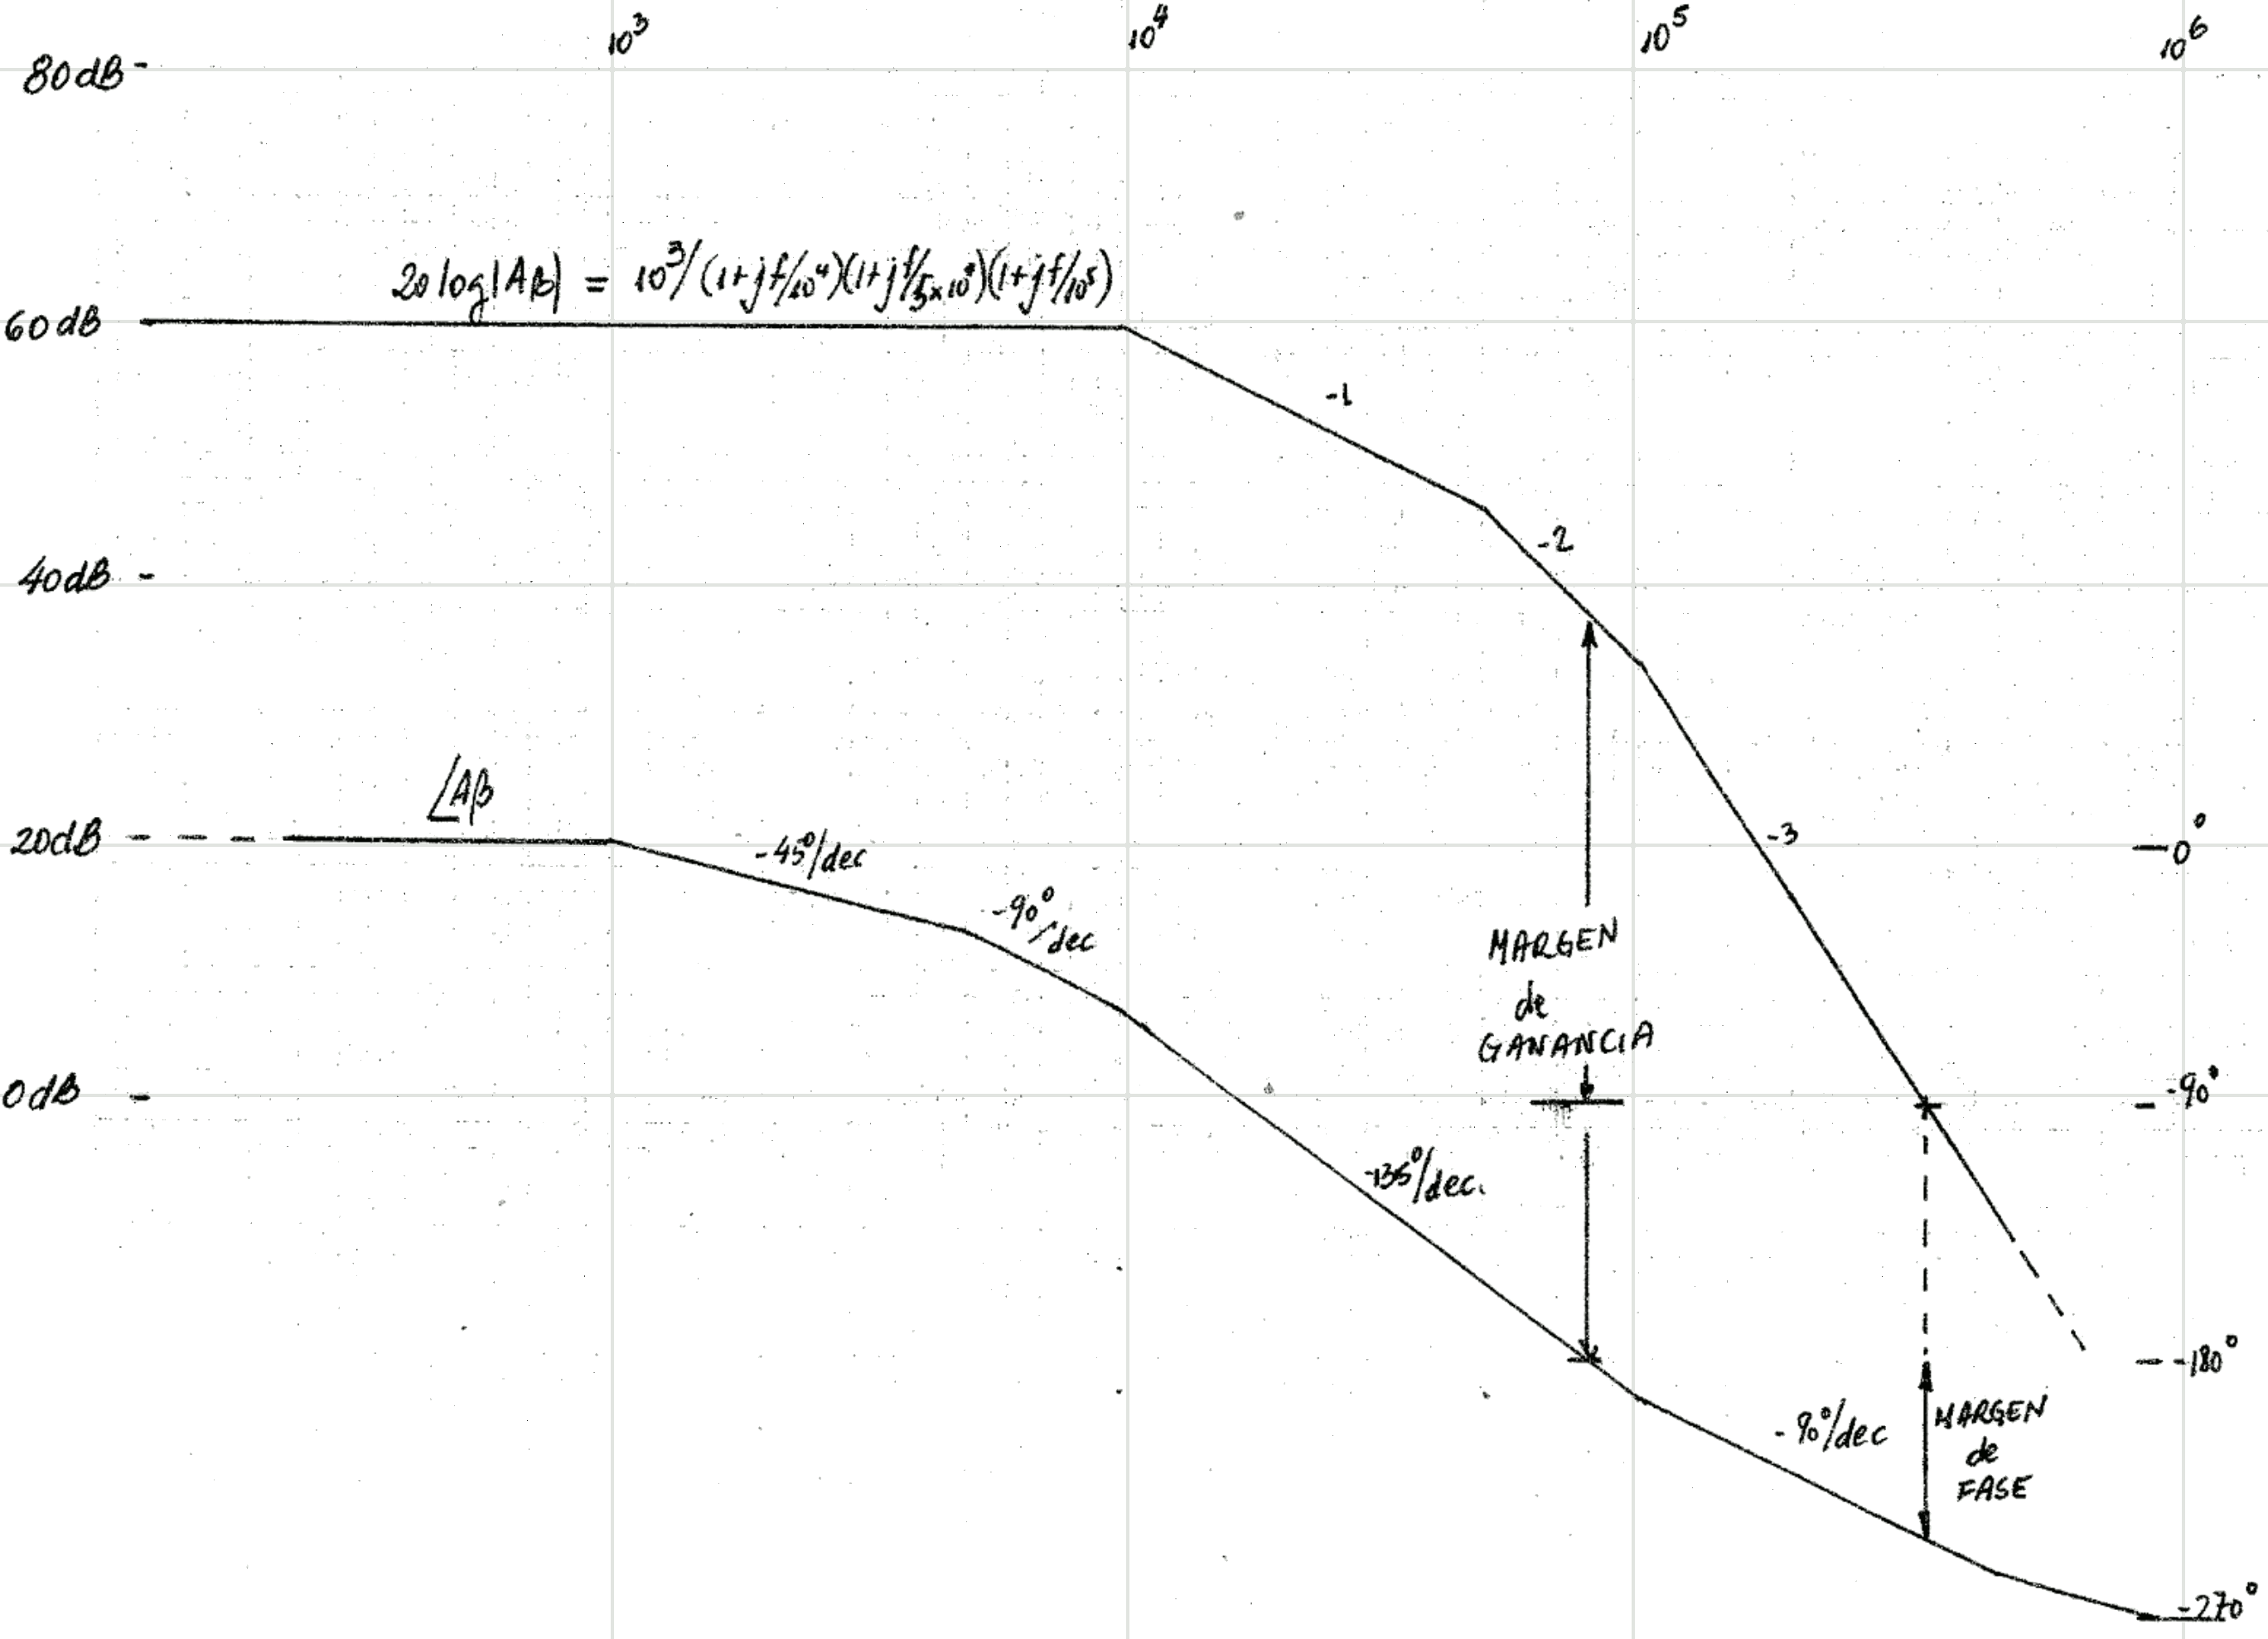
\includegraphics[width=0.96\linewidth]{_fig/osc_ejemplo1-bode.png}
	\caption{Diagrama de Bode el Ejemplo 1}
	\label{fig:osc_ejemplo1-bode}
\end{figure}

El criterio de Nyquist y el de Marge de Fase y de Ganancia coinciden en identificar este sistema con retroalimentación como inestable y con tendencia a oscilar.

\subsection{Modificaciones al producto AB} %p194

¿Como podemos convertir este sistema en un sistema estable?

Una opción es reducir la retroalimentación, es decir, reducir $\beta$. El valor máximo de $\beta$ puede encontrarse deslizando la gráfica de $20 \log |A_0 \beta|$ hacia abajo a medida que se disminuye $\beta$ hasta obtener los márgenes de fase y de ganancia deseados.

De esta manera, si $20 \log |A_0 \beta|$ se reduce a $\approx 12$ dB, habrá un margen de fase de $\approx 45^\circ$, y un margen de ganancia de aproximadamente 10 dB. Para que $20 \log |A_0 \beta|$ sea igual a 12 dB, quiere decir que $|A_0 \beta| = 4$, de donde $\beta = \frac{4}{A_0} = \frac{4}{100000} = 0.0004$.

O, el mismo resultado puede obtenerse al encontrar el valor de $A$ para un margen de fase de $\approx 45^\circ$, cuando $\angle A = -135^\circ$, llamémoslo $A_{135}$, y entonces el valor máximo de $\beta$ viene dado por:

\[
20 \log \beta = -20 \log |A_{135}|
\]

La justificación de este procedimiento deriva de que queremos un margen de $45^\circ$ cuando la ganancia $A \beta$ sea igual a $1$,

o \( 20 \log |A_{135} \beta| = 0 \)

o \( 20 \log |A_{135}| + 20 \log |\beta| = 0 \)

o \( 20 \log |\beta| = -20 \log |A_{135}| \)

Aplicando este procedimiento al Ejercicio 1, encontramos que para un margen de fase de $45^\circ$, se obtiene $20 \log |A_{135}| = 68$ dB, por lo tanto esto da $20 \log |\beta| = -68$ dB, o $\beta = 0.0004$, el mismo resultado anterior.

En resumen, una forma de hacer un sistema estable consiste en mantener $A$, pero modificar $\beta$ para garantizar el cumplimiento de las condiciones de estabilidad. Al cambiar $\beta$ de 1 al valor de 0.0004, un sistema inestable se convierte en uno estable.

De este ejercicio podemos hacer las siguientes observaciones:

\begin{itemize}
	\item La inestabilidad es más factible a medida que aumenta $\beta$, es decir, a medida que la ganancia del sistema con retroalimentación es más baja; con ganancias altas con retroalimentación presentan menos problemas;
	\item Sin embargo, normalmente uno no puede jugar con el valor de $\beta$, sobre todo porque de el depende la ganancia con retroalimentación que suele ser uno de las especificaciones del sistema global
\end{itemize}

Por lo tanto, si nos interesa un sistema estable y al mismo tiempo un valor especifico de $\beta$, entonces se requiere otra forma de modificar el sistema inestable. Una solución es la \textbf{Compensación de Frecuencia}, que consiste en modificar la respuesta de frecuencia del amplificador $A$, o de la red de retroalimentación $\beta$.

Tres tipos de compensación de frecuencia son:

\begin{description}
	\item[Compensación por atraso (polo dominante)] Se introduce un polo adicional en \( A \) a una frecuencia baja, para reducir la ganancia de \( A \) antes de alcanzar las frecuencias de los otros polos.
	\item[Compensación por adelanto] Se introduce un cero en la función de transferencia, añadiendo fase positiva para cumplir con el margen de fase requerido.
	\item[Compensación por adelanto-atraso] Se añade un polo y un cero, seleccionando el cero para cancelar el polo más bajo.
\end{description}

\subsection{Compensación de polo dominante} %p197

Se modifica el amplificador de modo que se agrega un polo dominante a una frecuencia muy por debajo a los demás polos en la función de transferencia. Por lo tanto, la ganancia disminuye a una tasa de \(-20 \, \text{dB/década}\) antes de llegar a la ganancia unitaria (\(0 \text{dB} \)) a una frecuencia donde los otros polos de $A$ aún no han contribuido notablemente al desfasamiento.

Se puede entender por qué esta técnica funciona al observar el lugar geométrico de las raíces para el circuito original y el circuito compensado, como se plantea en la Figura \ref{fig:osc_comp-polo-dominante}. Con la misma cantidad de retroalimentación, el desplazamiento de los polos aún no ha alcanzado las zonas cercanas al plano derecho.

\begin{figure}[h]
	\centering
	\subfloat[Circuito Original]
	{
		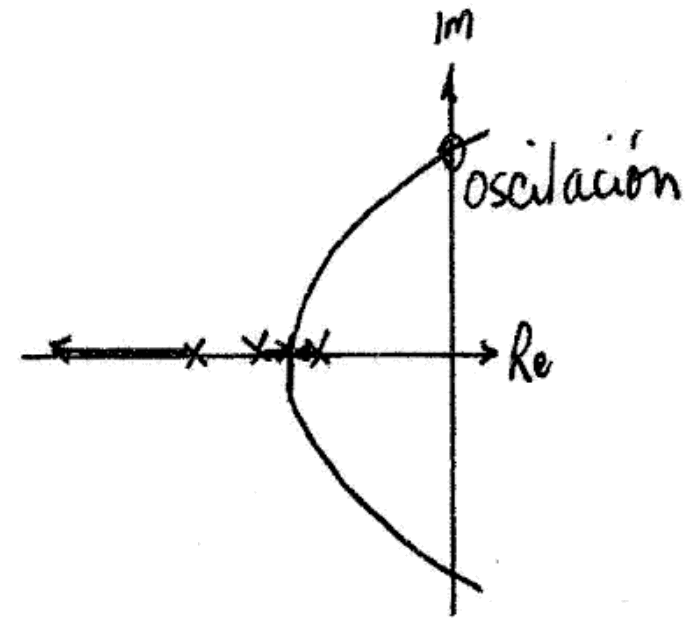
\includegraphics[width=0.45\linewidth]{_fig/osc_comp-polo-dominante_cto-original.png}
		\label{fig:osc_comp-polo-dominante_cto-original}
	}
	\subfloat[Circuito Compensado]
	{
		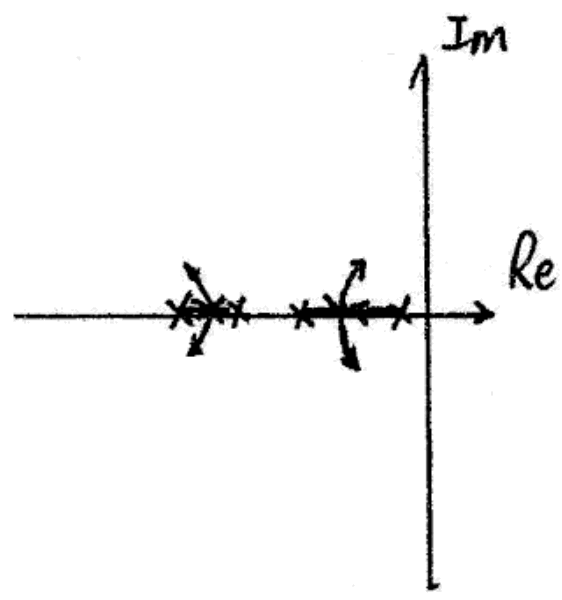
\includegraphics[width=0.45\linewidth]{_fig/osc_comp-polo-dominante_cto-compensado.png}
		\label{fig:osc_comp-polo-dominante_cto-compensado}
	}
	\caption{Efecto de Compensación de Polo Dominante Sobre el Lugar Geométrico de las Raíces}
	\label{fig:osc_comp-polo-dominante}
\end{figure}

Para determinar la frecuencia más indicada para el polo dominante se sigue el siguiente procedimiento:

\begin{enumerate}
	\item Ubicarse en el diagrama de Bode de \(A\beta\) en el punto correspondiente a \(0 \, \text{dB}\) y a la frecuencia del polo original más bajo.
	\item Desde ese punto, trazar una línea con pendiente de \(-20 \, \text{dB/década}\) hacia la izquierda (hacia frecuencias más bajas) hasta intersectar la gráfica de \(20 \log |A\beta|\).
	\item La frecuencia correspondiente a esta intersección es la frecuencia del polo dominante.
\end{enumerate}

El ancho de banda del sistema cerrado queda aproximadamente igual al valor del primer polo de la función original.

Por ejemplo, si se vuelve a la función de transferencia del Ejemplo 1, inicialmente no compensada, el producto \(A\beta\) daba lugar a un sistema inestable. Si se aplica esta técnica de compensación por polo dominante, se obtiene una intersección de la recta a la frecuencia de \(10\text{Hz}\), tal como se muestra en la Figura \ref{fig:osc_comp-polo-dominante_ubicacion-polo-dominante}. Nos queda la siguiente función de transferencia.

\[
A(s) = \frac{1000}{(1 + j f / 10^4)(1 + j f / 10)(1 + j f / 5 \times 10^4)(1 + j f / 10^5)}
\]

\begin{figure}[h]
	\centering
	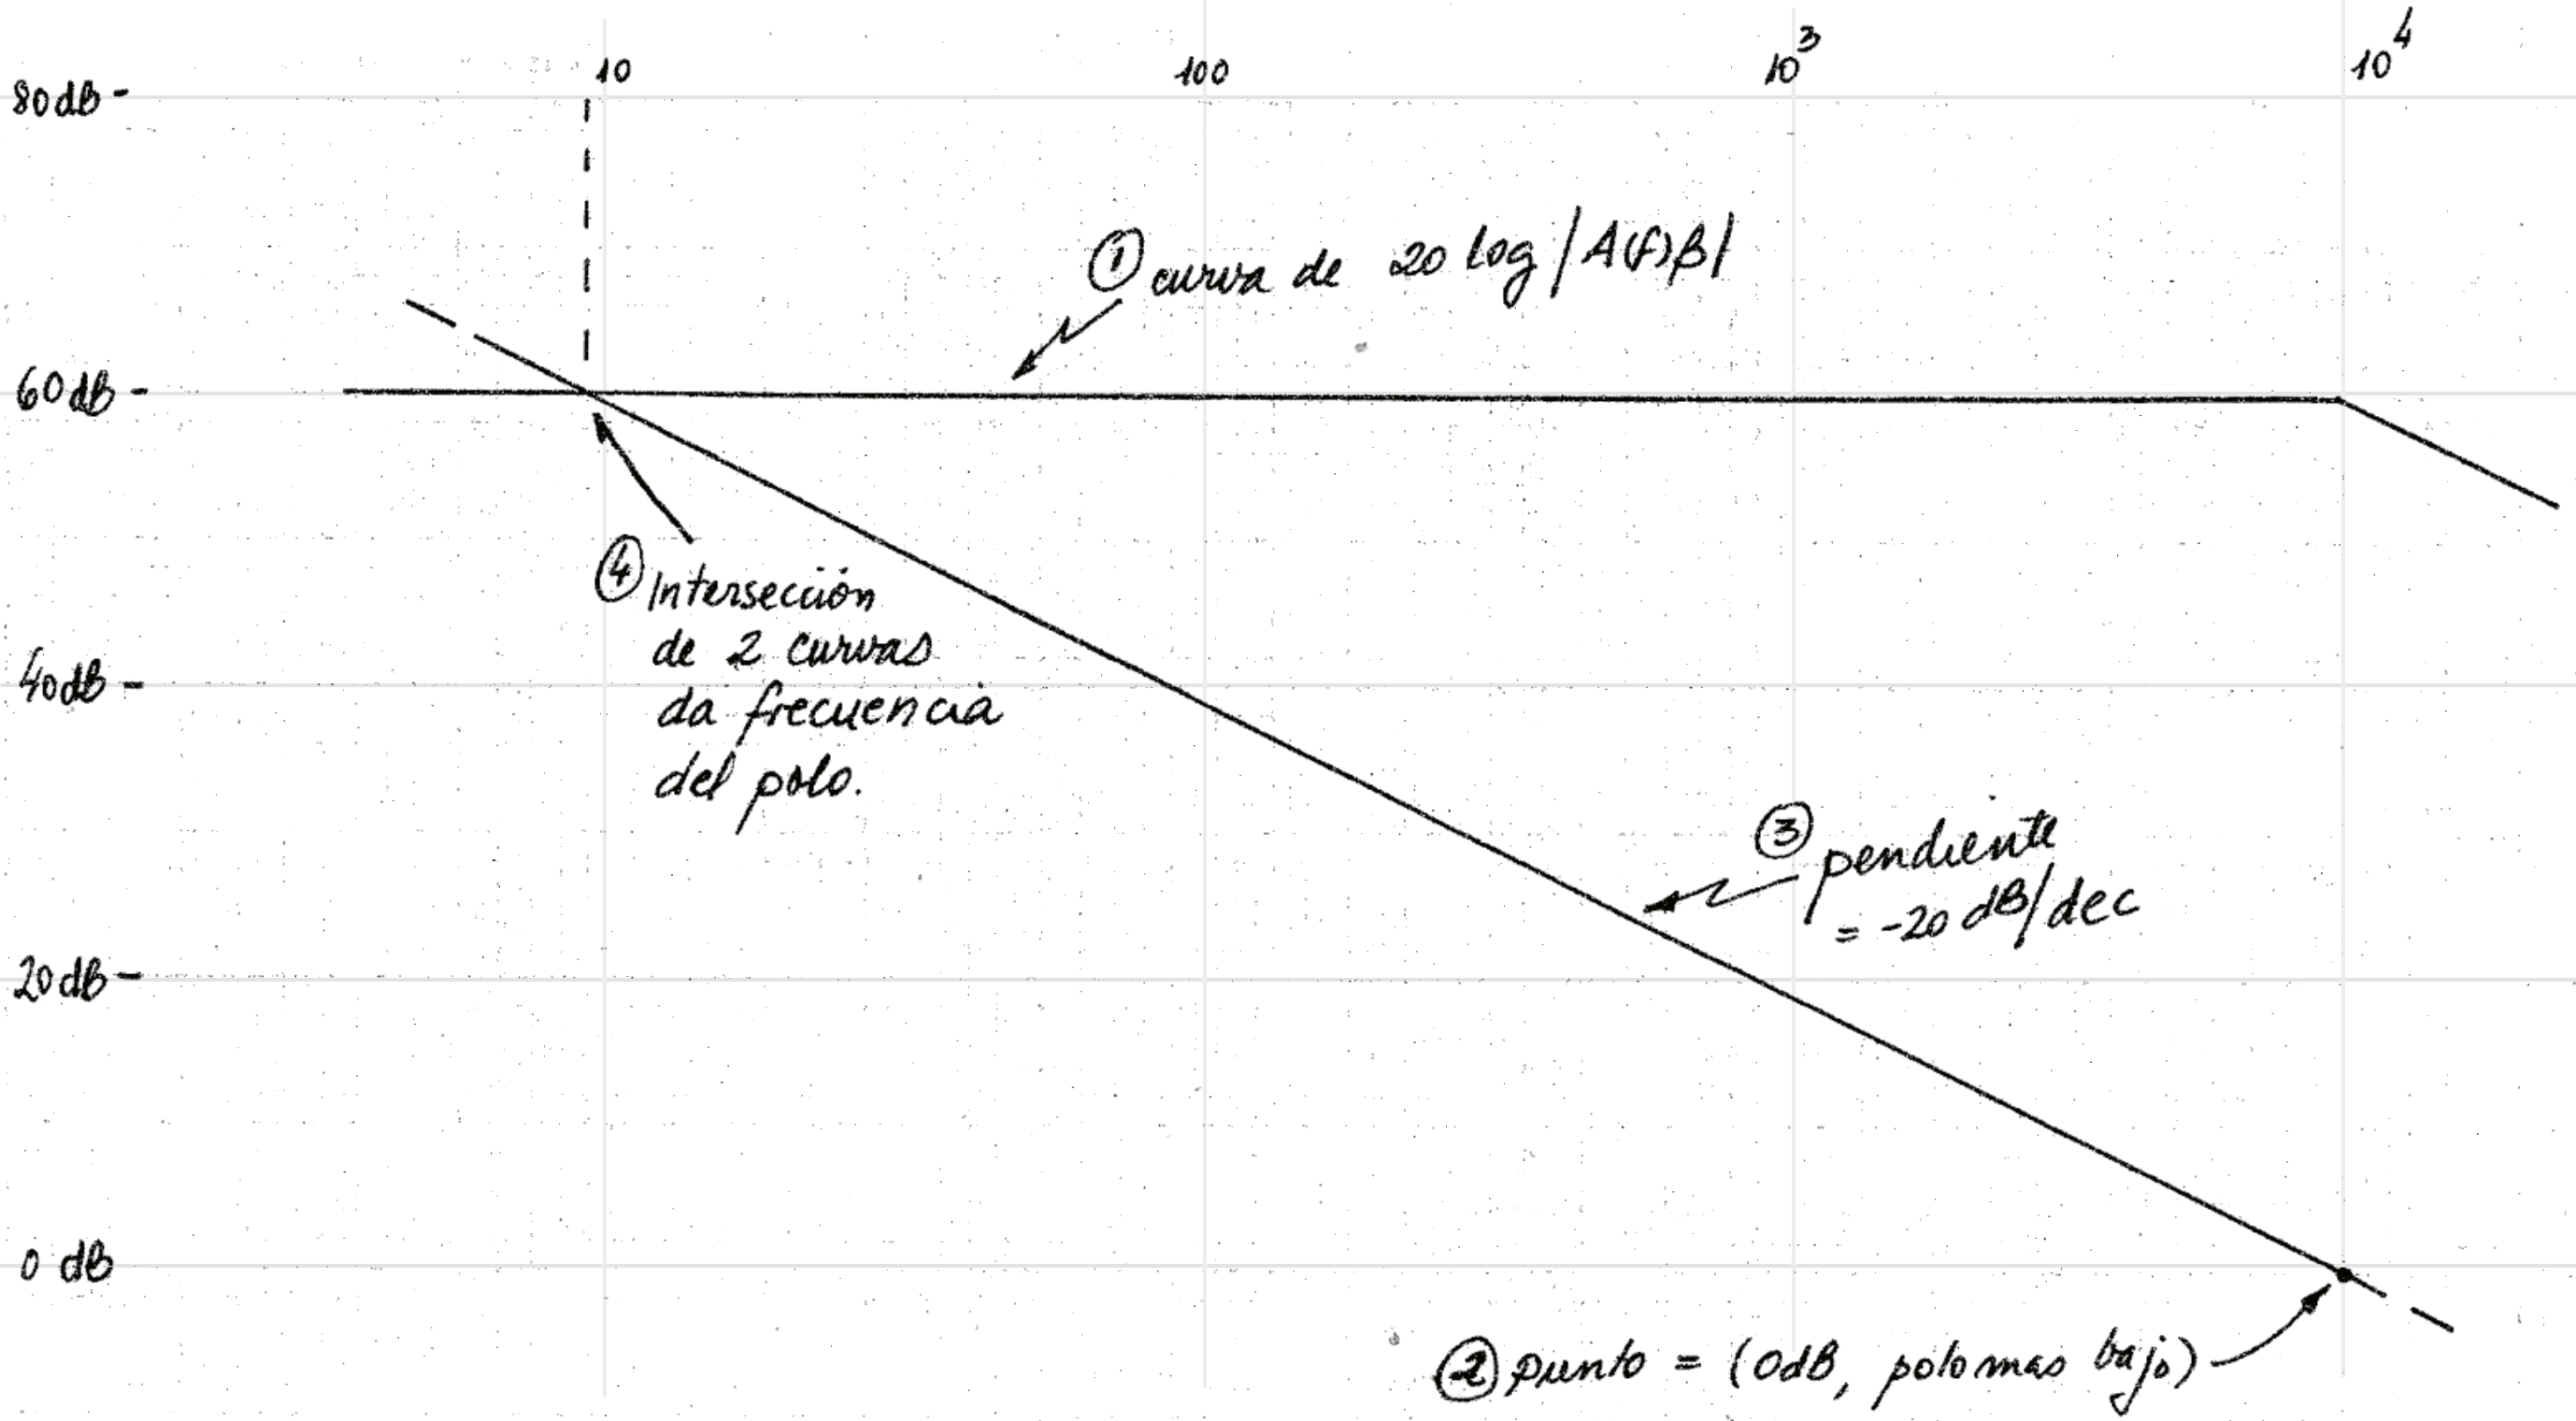
\includegraphics[width=0.96\linewidth]{_fig/osc_comp-polo-dominante_ubicacion-polo-dominante.png}
	\caption{Ubicación de Frecuencia de Polo Dominante}
	\label{fig:osc_comp-polo-dominante_ubicacion-polo-dominante}
\end{figure}

El Diagrama de Bode correspondiente se muestra en la Figura \ref{fig:osc_comp-polo-dominante_ab-compensado}, donde se observa que el margen de ganancia y de fase indican que el sistema es estable.

\begin{figure}[h]
	\centering
	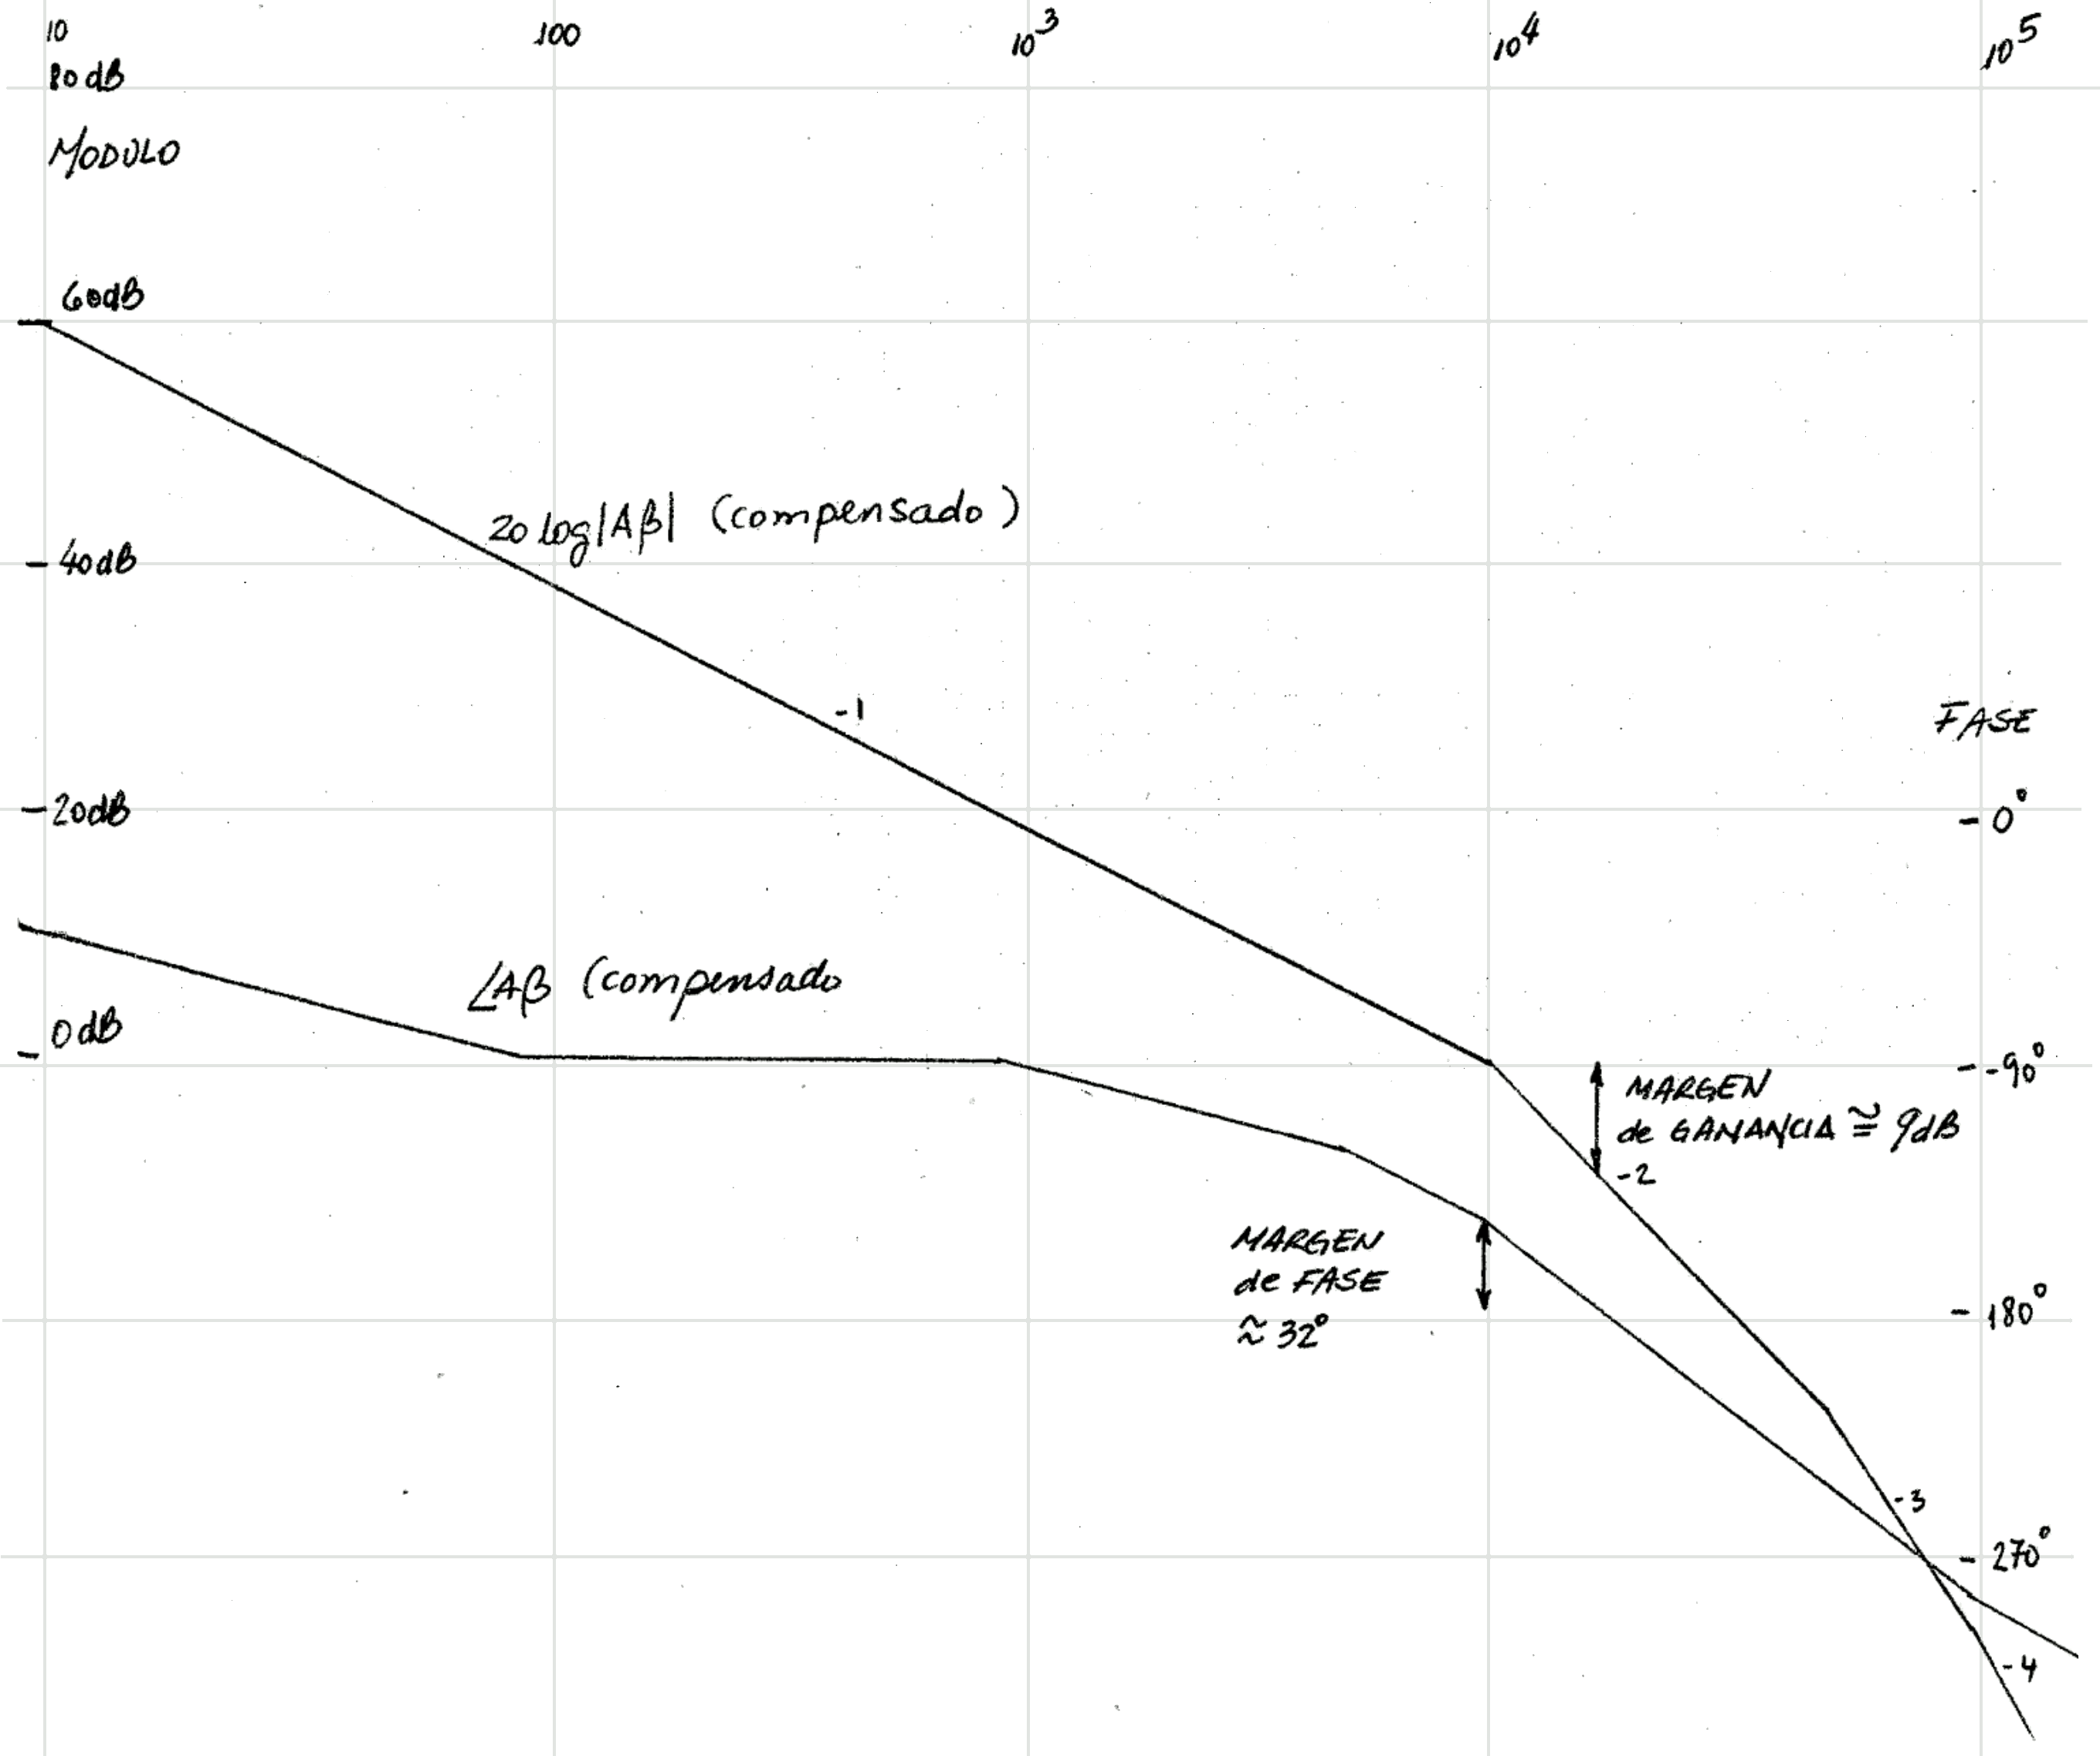
\includegraphics[width=0.96\linewidth]{_fig/osc_comp-polo-dominante_ab-compensado.png}
	\caption{Producto \(A\beta\) compensado}
	\label{fig:osc_comp-polo-dominante_ab-compensado}
\end{figure}

La \textbf{compensación por polo dominante} es una técnica utilizada para estabilizar amplificadores operacionales, como el 741. Aunque se puede determinar la frecuencia del polo usando un análisis preciso de la respuesta de frecuencia del amplificador, esto no siempre es necesario. Basta con asegurarse de que la frecuencia del polo sea lo suficientemente baja, ya que mientras más bajo sea el polo, mayor será la estabilidad.

Para compensar un amplificador inestable, como el ilustrado en la Figura \ref{fig:osc_comp-polo-dominante_sch}, el polo se puede introducir de varias formas:

\begin{itemize}
	\item Colocando un condensador \textbf{grande} entre el colector y la base de \(Q_1\), \(Q_2\) o \(Q_3\) y.
	\item Colocando un condensador grande entre la base de \(Q_1\) y tierra.
\end{itemize}

Estas técnicas permiten modificar el comportamiento de frecuencia del circuito y mejorar su estabilidad.

\begin{figure}[h]
	\centering
	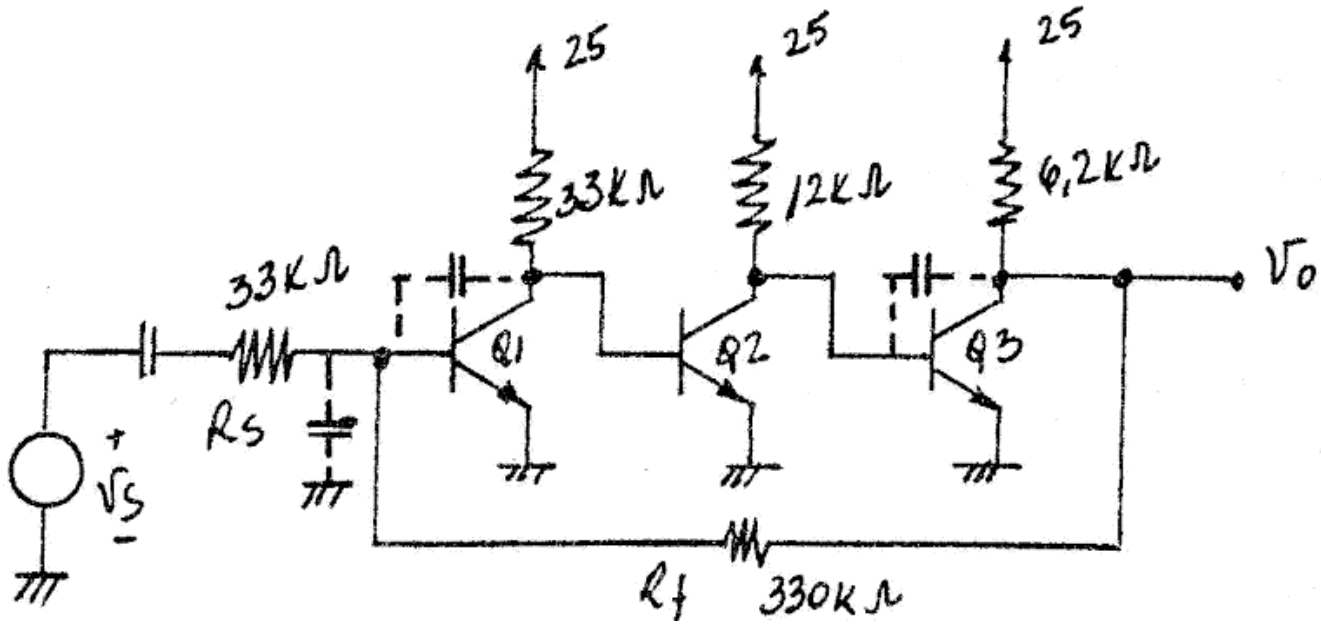
\includegraphics[width=0.96\linewidth]{_fig/osc_comp-polo-dominante_sch.png}
	\caption{Compensación de Frecuencia de Polo Dominante}
	\label{fig:osc_comp-polo-dominante_sch}
\end{figure}

Como una alternativa genérica para crear un polo dominante, se plantea la configuración de la Figura \ref{fig:osc_comp-polo-dominante_red-compensatoria}, en donde al amplificador básico de 3 polos se agrega un circuito RC a la salida. El polo creado viene dado por:

\[
f_p = \frac{1}{2\pi RC}
\]

Sujeto a la condición:

\[
R \gg Z_{o}(AV)
\]

\begin{figure}[h]
	\centering
	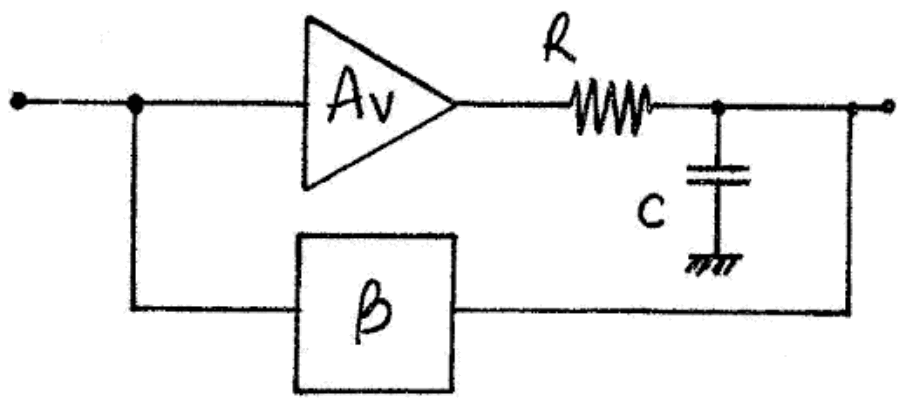
\includegraphics[width=0.96\linewidth]{_fig/osc_comp-polo-dominante_red-compensatoria.png}
	\caption{Amplificador con su red compensatoria de Polo Dominante}
	\label{fig:osc_comp-polo-dominante_red-compensatoria}
\end{figure}

La desventaja de esta técnica es que reduce enormemente el ancho de banda del amplificador. Las otras técnicas de compensación de frecuencia son más delicadas, pues exigen un conocimiento preciso de la respuesta de frecuencia, con la ventaja de que el ancho de banda resultante es mayor.

\subsection{Compensación por adelanto-atraso} %p202

Aquí se agrega un cero para cancelar el polo más pequeño y se introduce un polo a una frecuencia menor. De esta forma, puede admitirse una mayor cantidad de retroalimentación sin que esto conlleve a una oscilación.

Desde el enfoque de lugar geométrico de las raíces, se muestra un sistema sin compensación y otro con compensación en la Figura \ref{fig:osc_comp-adelanto-atraso}. Nuevamente, se logra el resultado deseado, es decir, un sistema estable para una cantidad determinada de retroalimentación.

\begin{figure}[h]
	\centering
	\subfloat[Sin Compensación]
	{
		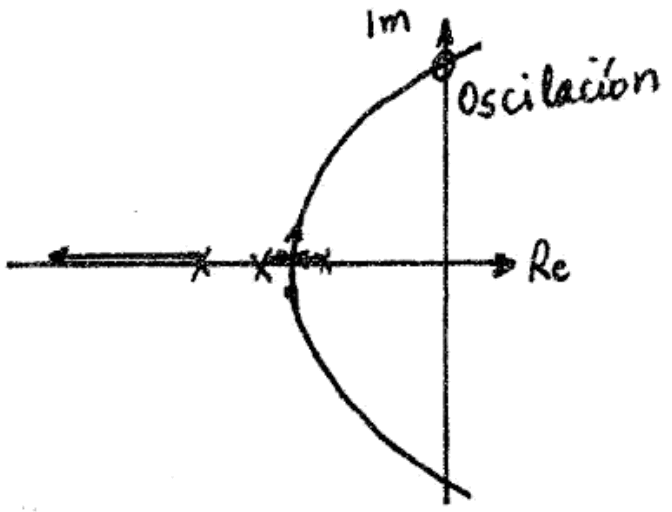
\includegraphics[width=0.45\linewidth]{_fig/osc_comp-adelanto-atraso_sin.png}
		\label{fig:osc_comp-adelanto-atraso_sin}
	}
	\subfloat[Con Compensación]
	{
		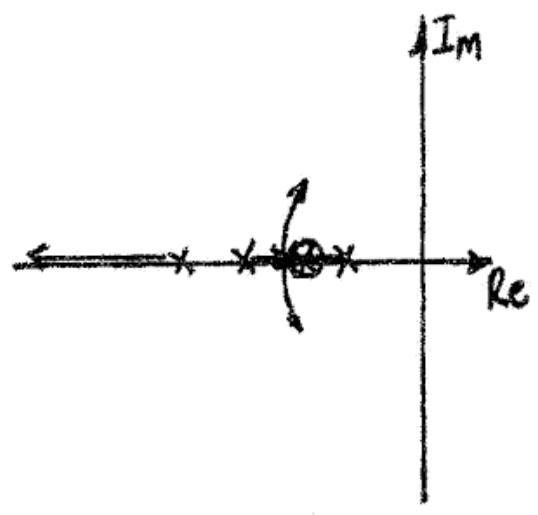
\includegraphics[width=0.45\linewidth]{_fig/osc_comp-adelanto-atraso_con.png}
		\label{fig:osc_comp-adelanto-atraso_con}
	}
	\caption{Efecto de Compensación de Polo Dominante Sobre el Lugar Geométrico de las Raíces}
	\label{fig:osc_comp-adelanto-atraso}
\end{figure}

Esta técnica permite que el sistema resultante tenga un ancho de banda mayor que lo que se obtiene con la técnica de polo dominante. Sin embargo, su aplicación es difícil, ya que, aunque el valor del cero no tiene que ser exactamente igual al del polo que se quiere cancelar, debe aproximarse bastante. De lo contrario, surgirá nuevamente la condición de inestabilidad.

En la Figura \ref{fig:osc_comp-adelanto-atraso_red-compensatoria} se indica como puede implementarse este tipo de compensación.

\begin{figure}[h]
	\centering
	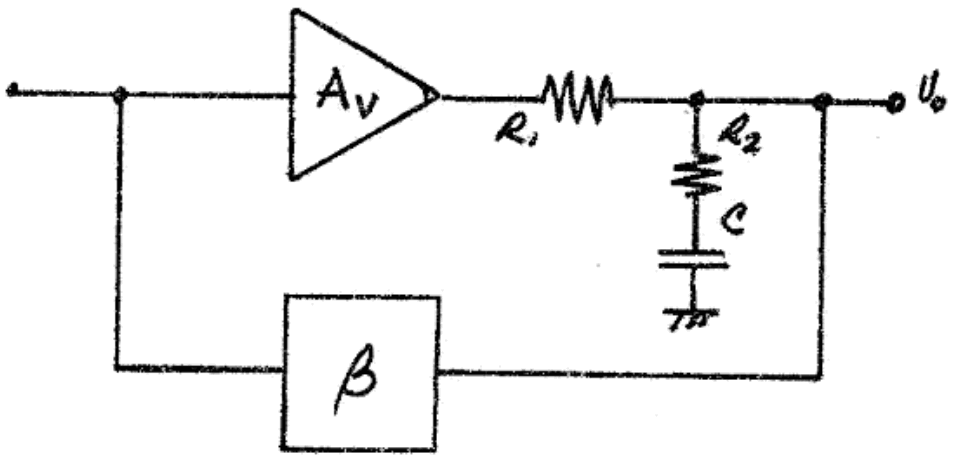
\includegraphics[width=0.96\linewidth]{_fig/osc_comp-adelanto-atraso_red-compensatoria.png}
	\caption{Compensación de Adelanto-Atraso}
	\label{fig:osc_comp-adelanto-atraso_red-compensatoria}
\end{figure}

Para ubicar el polo en esta técnica, se procede de forma idéntica al método planteado para el polo dominante, con la diferencia de que la pendiente arranca desde el segundo polo de la función de transferencia original.

Como ejemplo, se aplica a la función de transferencia del Ejemplo 1 y se obtiene la frecuencia de \(50\text{Hz}\) como lo ilustra la Figura \ref{fig:osc_comp-adelanto-atraso_ubicacion-polo-dominante}, y el Diagrama de Bode de \(A\beta\), la Figura \ref{fig:osc_comp-adelanto-atraso_ab-compensado}.

\begin{figure}[h]
	\centering
	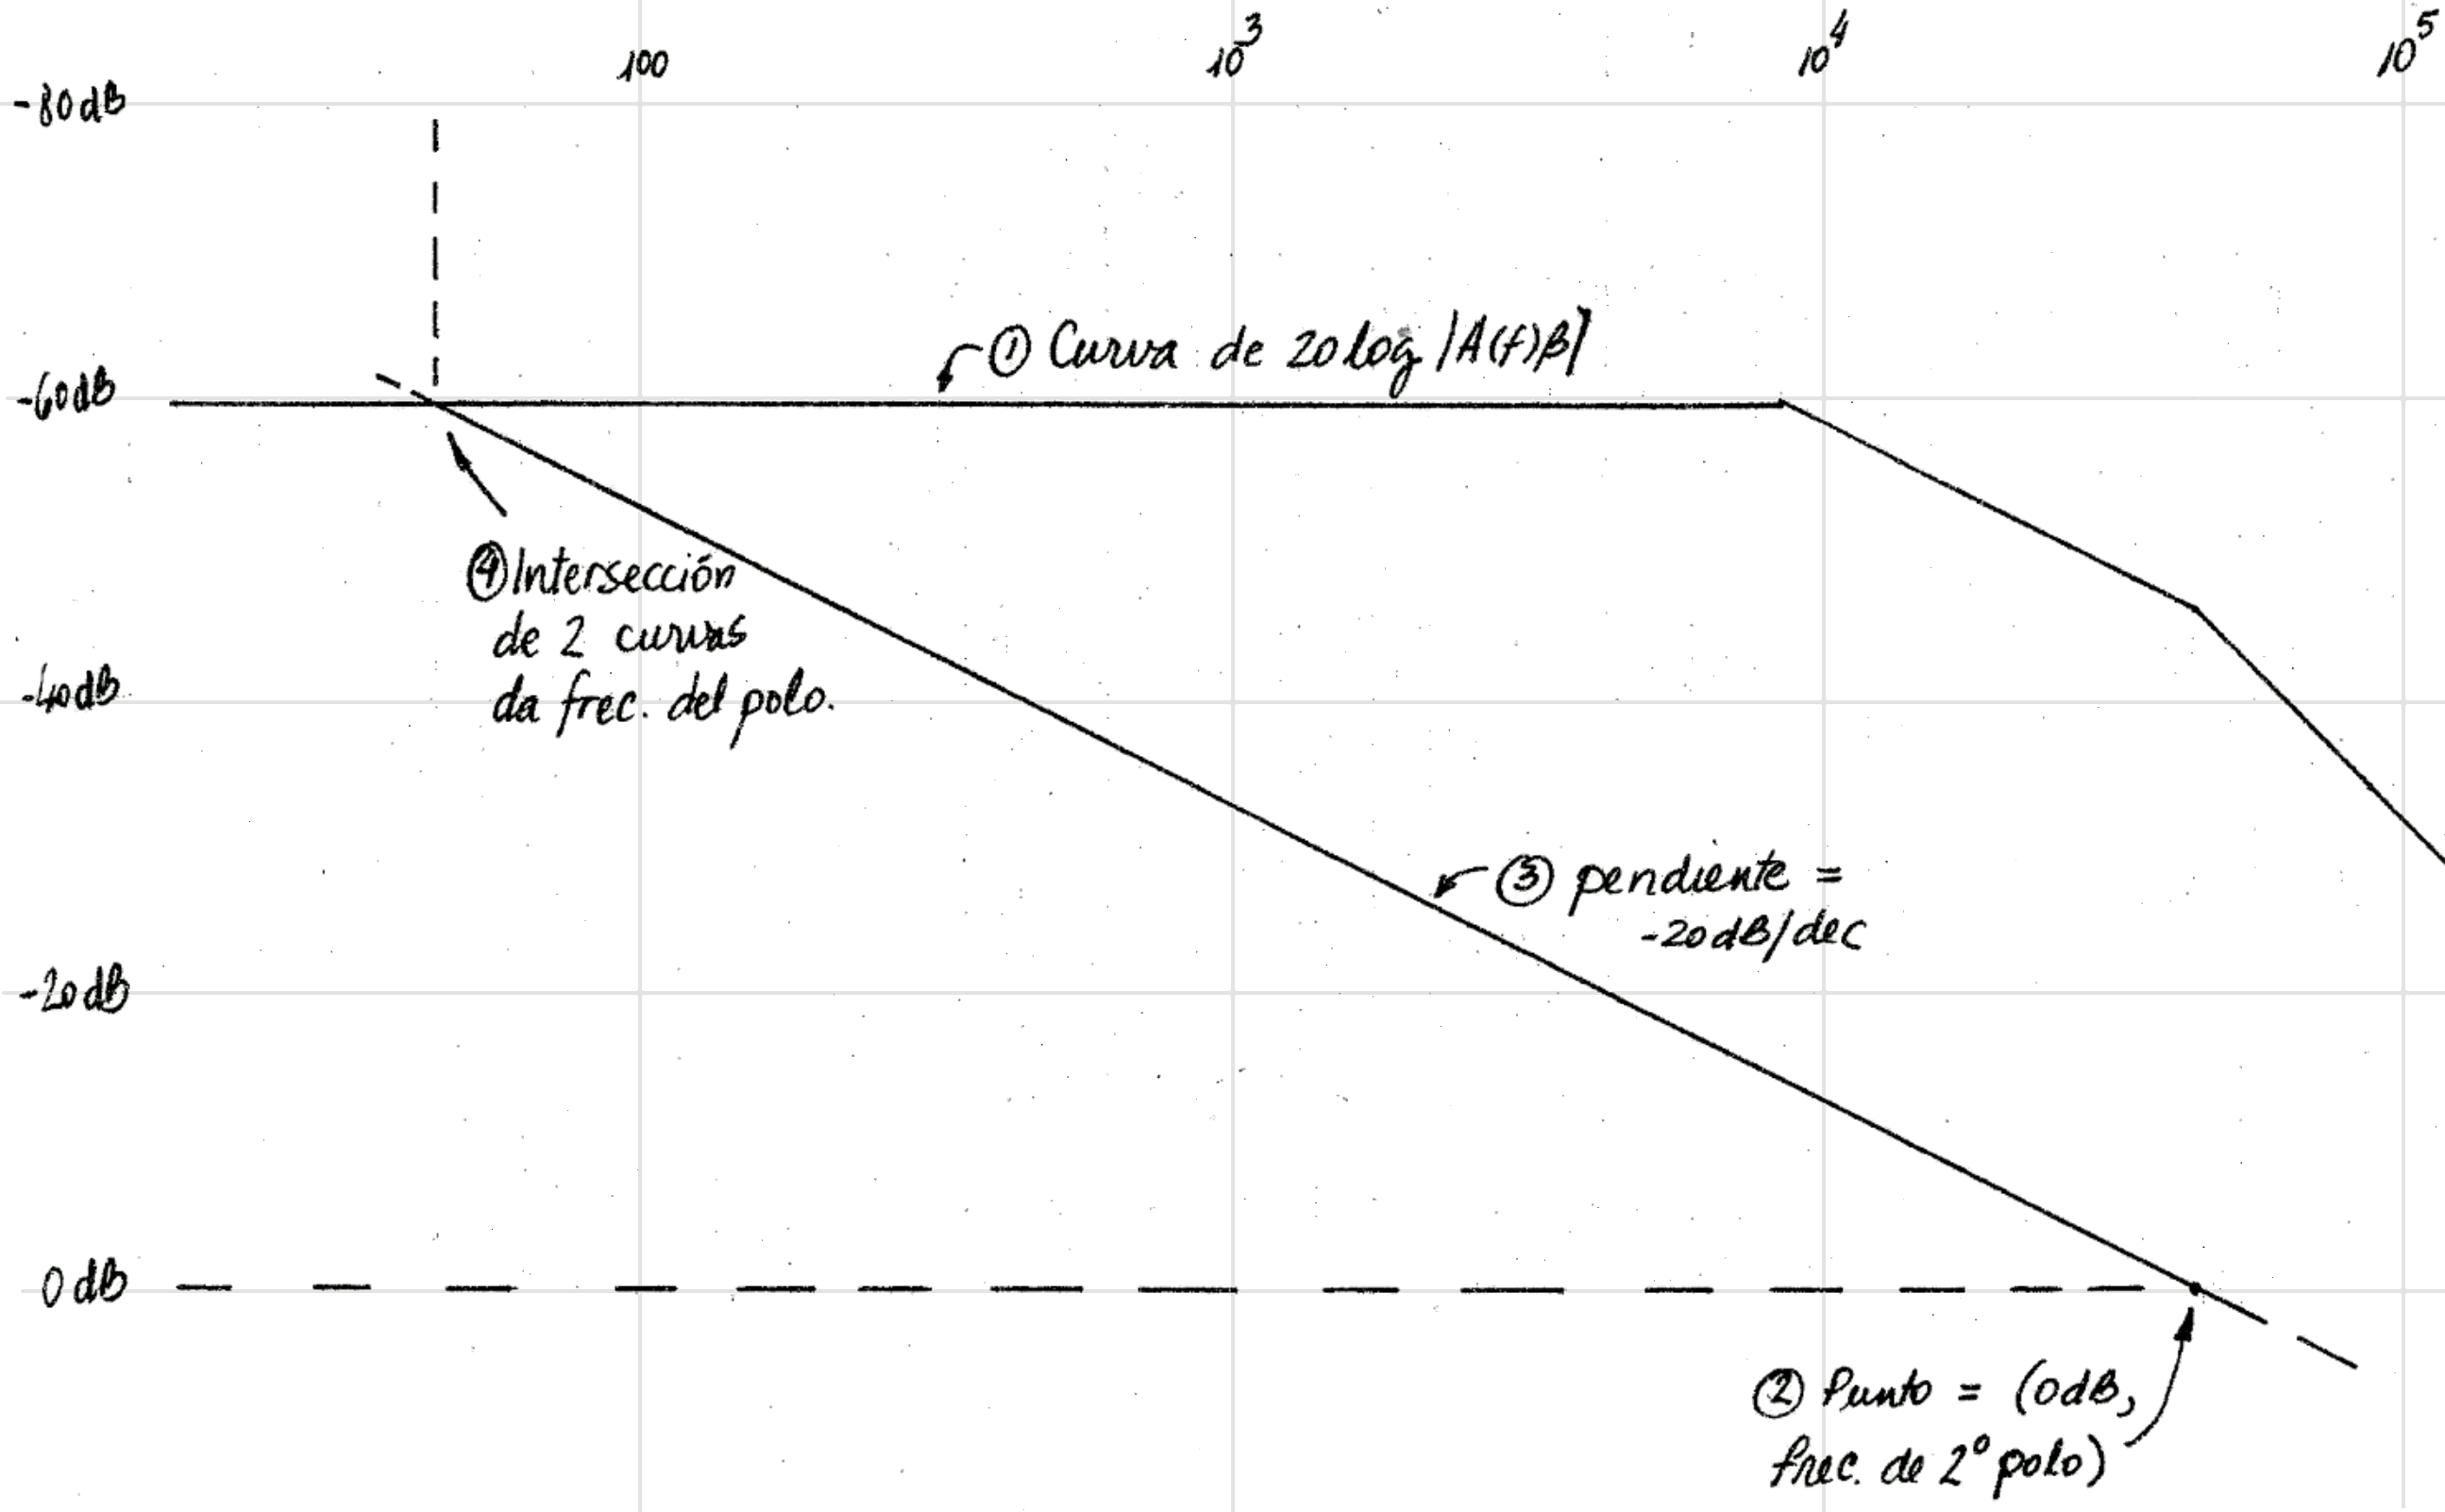
\includegraphics[width=0.96\linewidth]{_fig/osc_comp-adelanto-atraso_ubicacion-polo-dominante.png}
	\caption{Ubicación de Frecuencia de Polo Dominante}
	\label{fig:osc_comp-adelanto-atraso_ubicacion-polo-dominante}
\end{figure}

\begin{figure}[h]
	\centering
	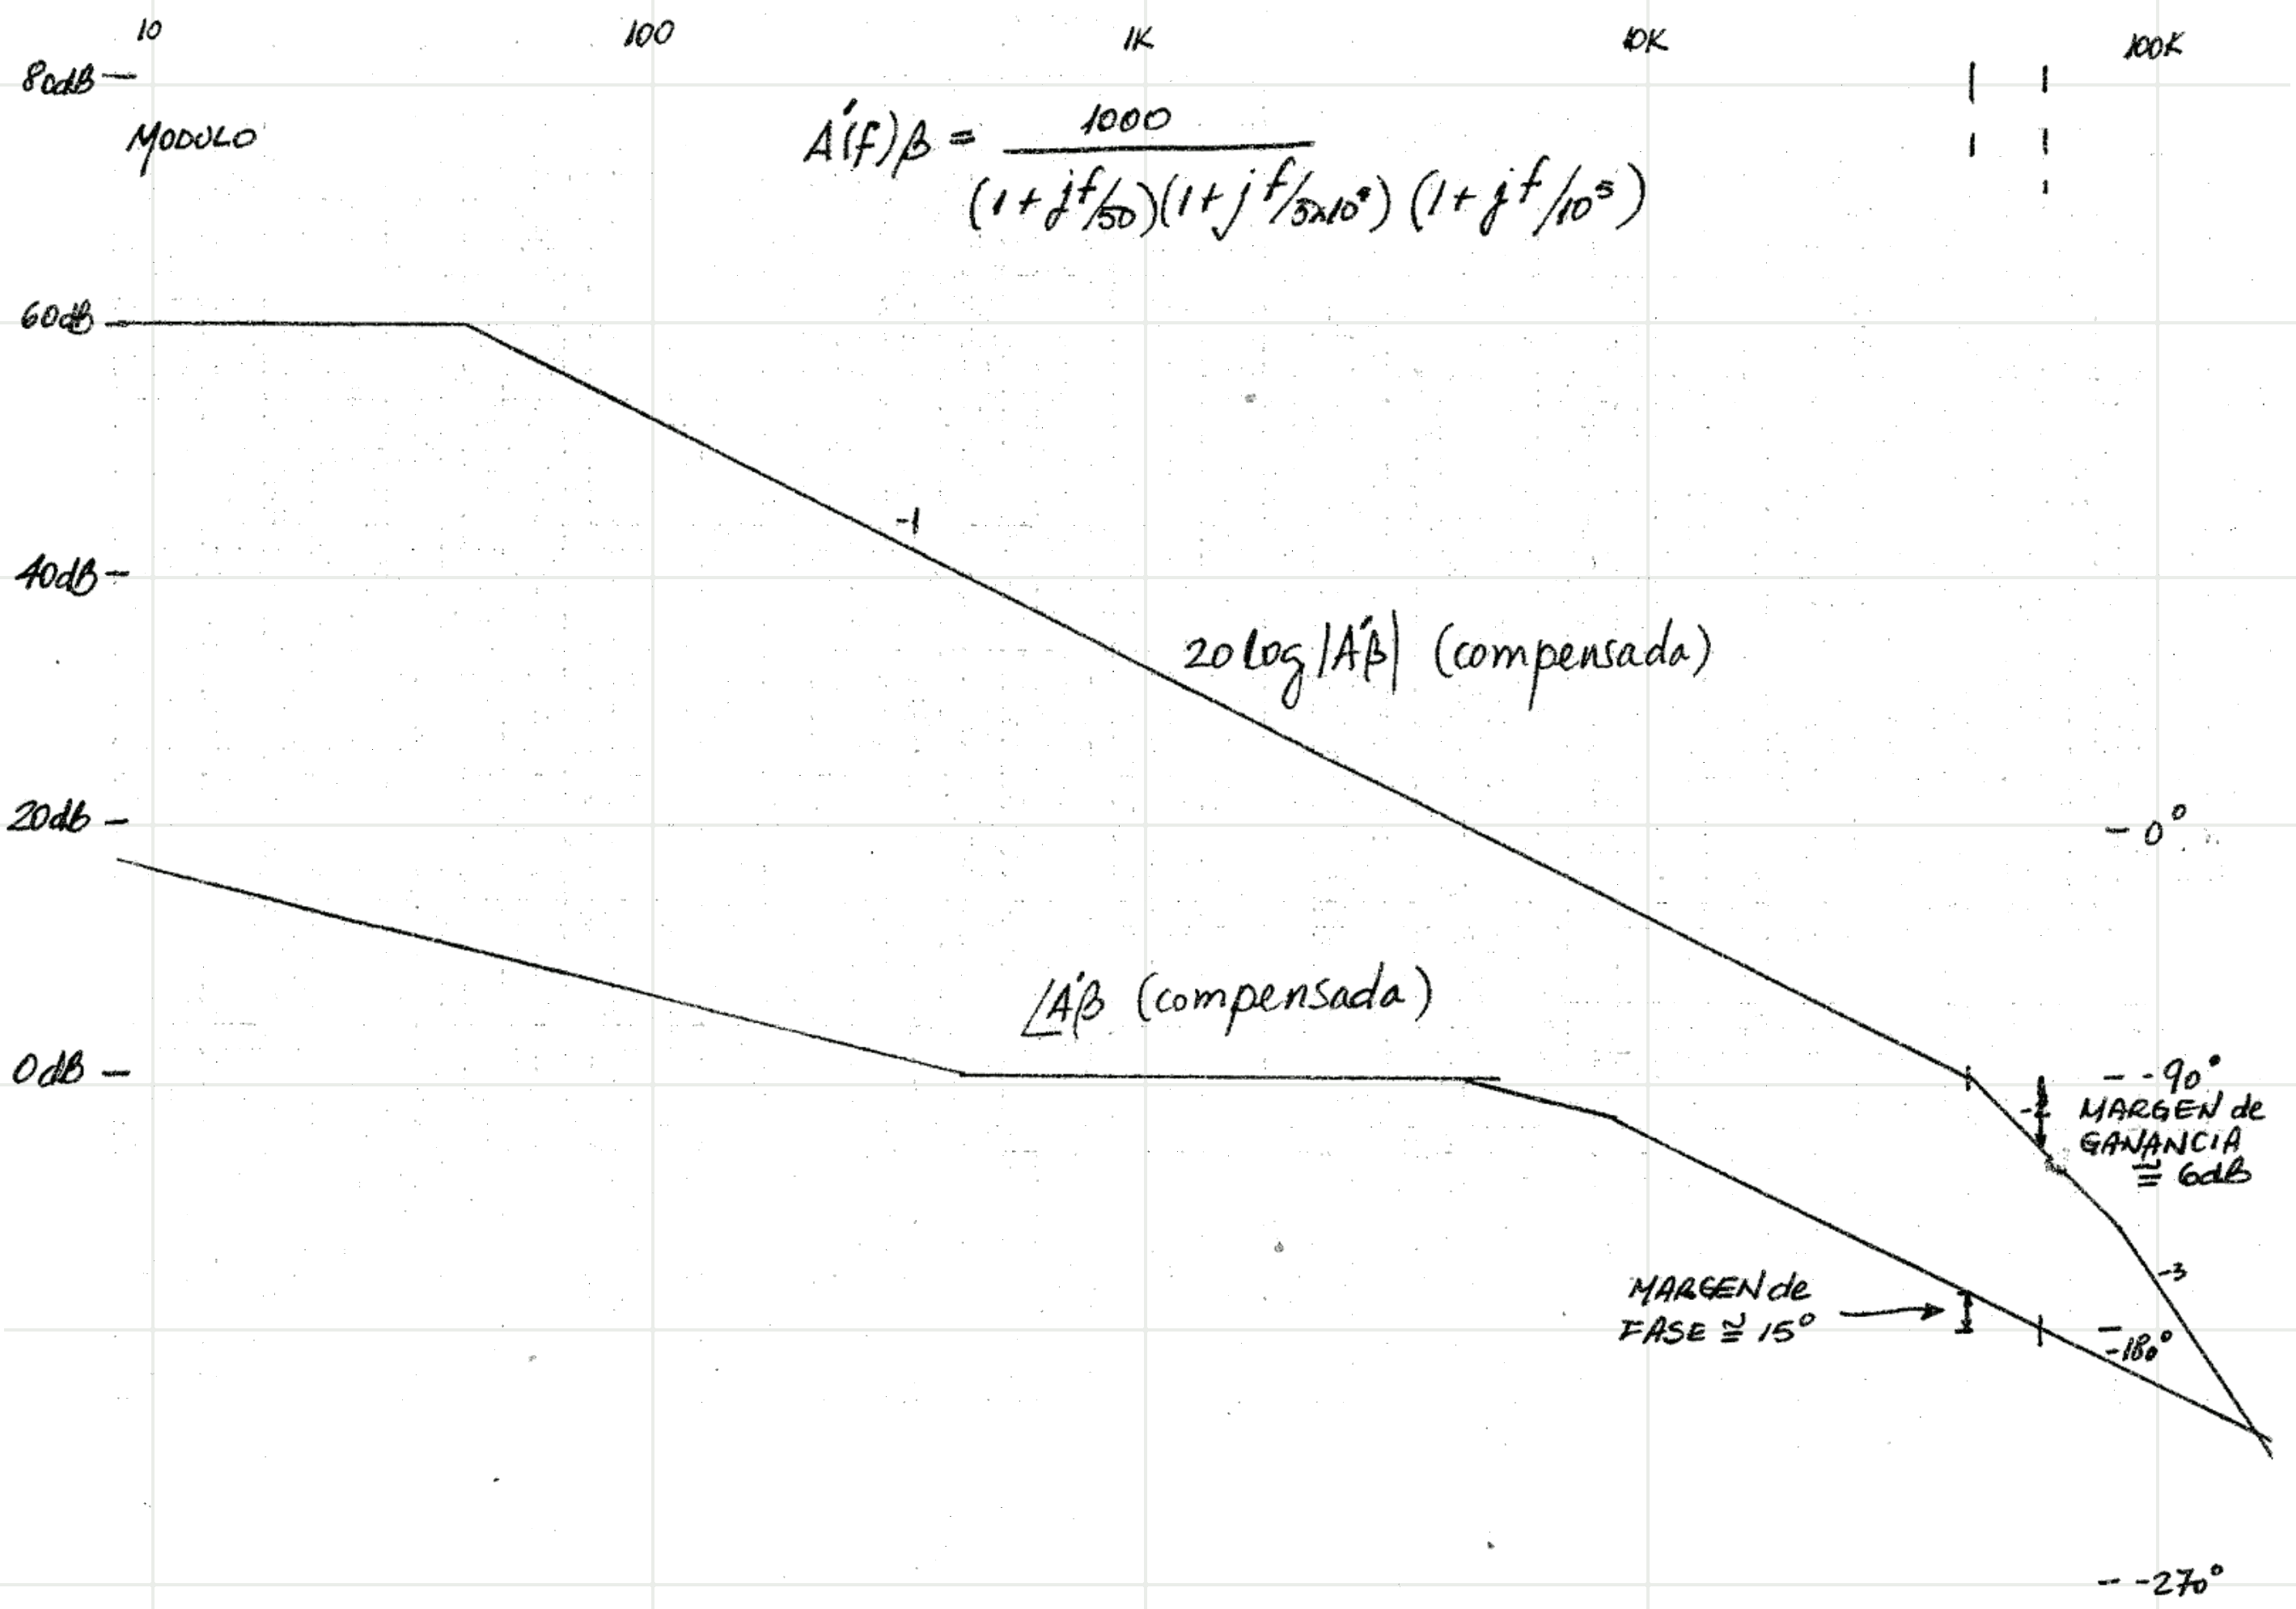
\includegraphics[width=0.96\linewidth]{_fig/osc_comp-adelanto-atraso_ab-compensado.png}
	\caption{Producto \(A\beta\) compensado}
	\label{fig:osc_comp-adelanto-atraso_ab-compensado}
\end{figure}

\subsection{Compensación por adelanto} %p206

En lugar de modificar la respuesta del amplificador sin retroalimentación, se puede optar por modificar la red de retroalimentación.

Por ejemplo, si volvemos al amplificador de tres etapas y le agregamos un condensador en paralelo con la resistencia de retroalimentación, como se muestra en la Figura \ref{fig:osc_comp-adelanto_sch}, se obtiene:

\[
\beta = \frac{I_f}{V_o} = -(G_f + sC_f)
\]

\begin{figure}[h]
	\centering
	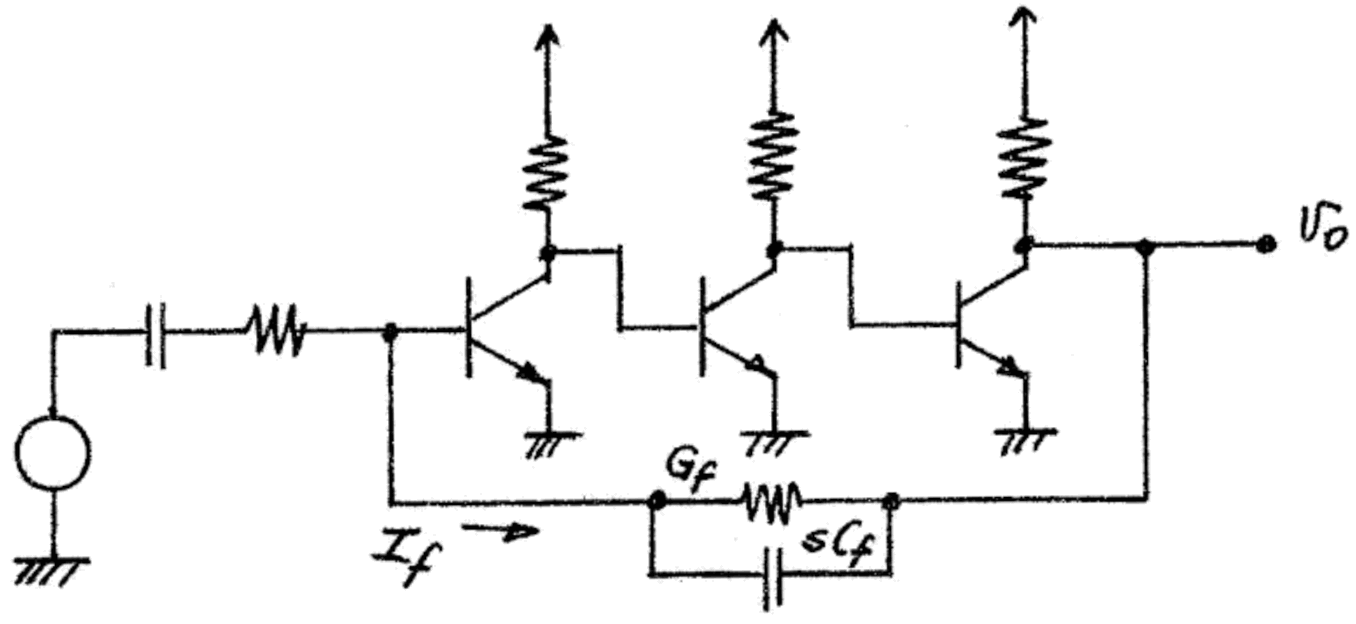
\includegraphics[width=0.96\linewidth]{_fig/osc_comp-adelanto_sch.png}
	\caption{Compensación por Adelanto - Modificando la Red de Retroalimentación}
	\label{fig:osc_comp-adelanto_sch}
\end{figure}

Por lo tanto,

\[
\beta A = -A(G_f + s C_f);
\]

es decir, se ha anexado un cero a la respuesta de frecuencia \(\beta A\). En el Diagrama de Bode de \(A \beta\), especialmente en relación con la fase, este cero proporciona una fase positiva de \(90^\circ\). Si se ubica adecuadamente, establecerá el margen de fase requerido para la estabilidad. Es recomendable ubicar este cero en la frecuencia donde la función de transferencia del amplificador (\(A\)) tiene un desfase de \(180^\circ\), o donde el sistema con retroalimentación, sin oscilar, presenta un pico en su respuesta de frecuencia.

Para el circuito anterior, la frecuencia de oscilación ocurrió a \(3 \text{MHz}\). Dado \(R_f = 330 \text{K}\Omega\), el valor adecuado de \(C_f\) viene dado por:

\[
C_f = \frac{1}{2\pi \cdot 330k \cdot 3 \times 10^6} = 0.6 \times 10^{-12} \text{F}
\]

Este valor es demasiado pequeño, ya que el valor mínimo disponible como elemento discreto es de \(3 \text{pF}\) (aproximadamente 20 veces más grande). Esta capacitancia es del mismo orden de magnitud que la capacitancia parasitaria natural entre los terminales de \(R_f\), lo cual dificulta el control preciso. Sin embargo, el procedimiento indicado es correcto.

\subsubsection{Ejemplo 2}

\textbf{Dado:}

\[
A(s) = \frac{10000}{(1 + j/10^4)(1 + j/10^5)(1 + j/5 \cdot 10^5)}
\]

\begin{enumerate}
	\item[a)] Aplique el criterio de Nyquist para determinar si el sistema es estable con \(\beta = 0.1\).
	\item[b)] Grafique \(|A|\) y \(\angle A\).
	\item[c)] Determine el valor máximo de \(\beta\) para garantizar un margen de fase de \(-45^\circ\).
	\item[d)] Aplique la técnica de compensación de frecuencia de polo dominante para garantizar estabilidad con \(\beta = 1\). Determine el ancho de banda del amplificador con retroalimentación.
	\item[e)] Aplique la técnica de compensación por adelanto-atraso para tener un sistema estable dado \(\beta = 0.01\).
	\item[f)] Repita el inciso anterior con la técnica de compensación por adelanto.
\end{enumerate}

\subsubsection{Ejemplo 3}

Trace la respuesta de frecuencia del amplificador de la Figura 4.12 sin retroalimentación. Los transistores son del tipo 2N3904. ¿Oscila? Determine una compensación de frecuencia adecuada para estabilizarlo.

\section{Osciladores} %p208

Ahora procuremos diseñar un circuito para oscilar a una frecuencia determinada. Por lo que hemos visto, bien podría funcionar un circuito que no tuviera condensador externo, sino que trabajara con las mismas capacitancias intrínsecas de los transistores o FET u operacionales. Sin embargo, y tal vez por ser estas capacitancias de valor desconocido o no confiable, se prefiere utilizar otras configuraciones con una estructura formal compuesta por RC externas y conocidas.

En cualquier caso, la condición de oscilación puede desprenderse de la expresión del amplificador con retroalimentación, $\frac{A}{1+A\beta}$. Si $1+A\beta = 0$, $\sigma^A\beta = -1$, $\sigma^{-A}\beta = 1$, entonces la ganancia en lazo cerrado se hace infinita, y tenemos un oscilador. En particular, la condición de que la ganancia de lazo, $-A\beta$, es igual a $+1$, es conocida como el criterio de Barkhausen. Sin una señal externa, la misma retroalimentación suministra la señal para mantener la oscilación: de la Figura \ref{fig:osc_oscilador}, una señal $x$ genera $Ax$ que produce $\beta Ax$ que regresa al punto de partida como $-A\beta x$, pero si $-A\beta = 1$, se regenera la misma señal original.

\begin{figure}[h]
	\centering
	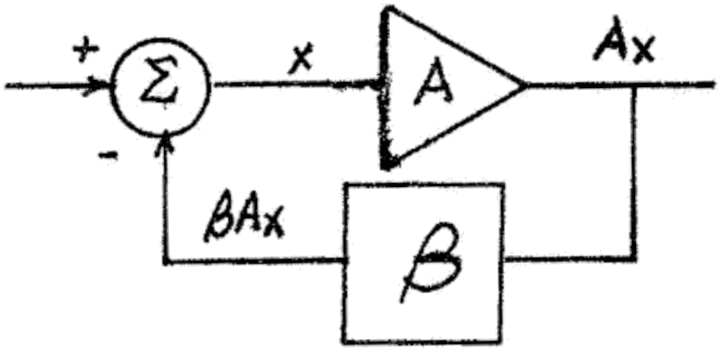
\includegraphics[width=0.8\linewidth]{_fig/osc_oscilador.png}
	\caption{Oscilador}
	\label{fig:osc_oscilador}
\end{figure}

En la práctica, $-\phi$ se hace ligeramente mayor que uno para garantizar un margen y evitar que se desvanezca la señal. Al mismo tiempo, se requiere un limitador "suave" para mantener la señal a un cierto nivel.

\subsection{Oscilador desplazamiento de fase} %p209

Un ejemplo de este tipo de oscilador se muestra en la Figura \ref{fig:osc_desplazamiento-de-fase}. Aquí cada celda RC aporta un desfasaje entre $\theta'$ y $\phi\theta'$, con una pequeña atenuación. Con las tres celdas, podemos lograr un desfasaje de $180^\circ$. Este desfasaje de $\beta$, más el desfasaje de $180^\circ$ de $(-A)$, nos proporcionan un desfasaje total de $360^\circ$ o $\theta'$, y si $A$ se escoge apropiadamente, se cumple la condición de Barkhausen.

\begin{figure}[h]
	\centering
	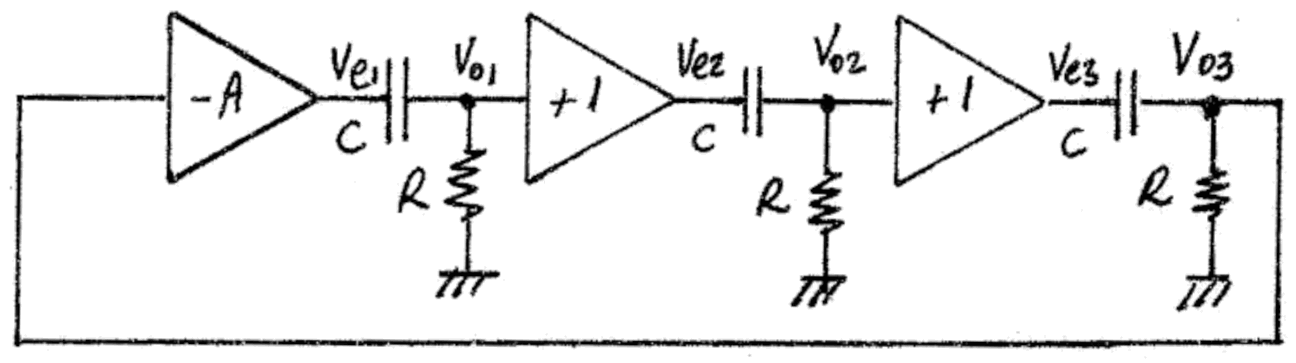
\includegraphics[width=0.8\linewidth]{_fig/osc_desplazamiento-de-fase.png}
	\caption{Oscilador Desplazamiento de Fase}
	\label{fig:osc_desplazamiento-de-fase}
\end{figure}

Como las tres celdas RC son iguales, para obtener un desfasaje de $180^\circ$ (quiero decir que cada celda aporta $\delta\theta'$), la función de transferencia de cada celda viene dada por:

\[
\frac{v_{o}}{v_{e}} = \frac{R}{R + \frac{1}{j\omega C}} = \frac{1}{1 + \frac{1}{j\omega RC}}
\]

\[
\frac{1}{1-\frac{1}{j\omega RC}}
\]

cuya fase es $\theta = \tan^{-1}\left(\frac{1}{\omega RC}\right)$; varía entre $90^\circ$ y $0^\circ$.

Si se fija $\theta = +60^\circ$, nos queda $\frac{1}{\omega RC} = \tan 60^\circ = \sqrt{3}$ y la expresión para la frecuencia de oscilación termina siendo:

\[
\omega = \frac{1}{\sqrt{3}}RC
\]

A esa frecuencia, el módulo de cada celda viene dada por:

\[ 
\left| \frac{v_0}{v_e} \right| = \frac{1}{\sqrt{1 + \frac{1}{(\omega RC)^2}}} = \frac{1}{\sqrt{4}} = \frac{1}{2} 
\]

Por ser tres celdas idénticas, la atenuación total viene dada por la atenuación de una elevada al cubo, lo que en este caso da $1/8$. Por lo tanto, $A$ tiene que ser ligeramente mayor que $1/(1/8) = 8$.

El mismo objetivo puede lograrse con circuitos RC directamente acoplados, como se muestra en la Figura \ref{fig:osc_desplazamiento-de-fase-1opamp}.

\begin{figure}[h]
	\centering
	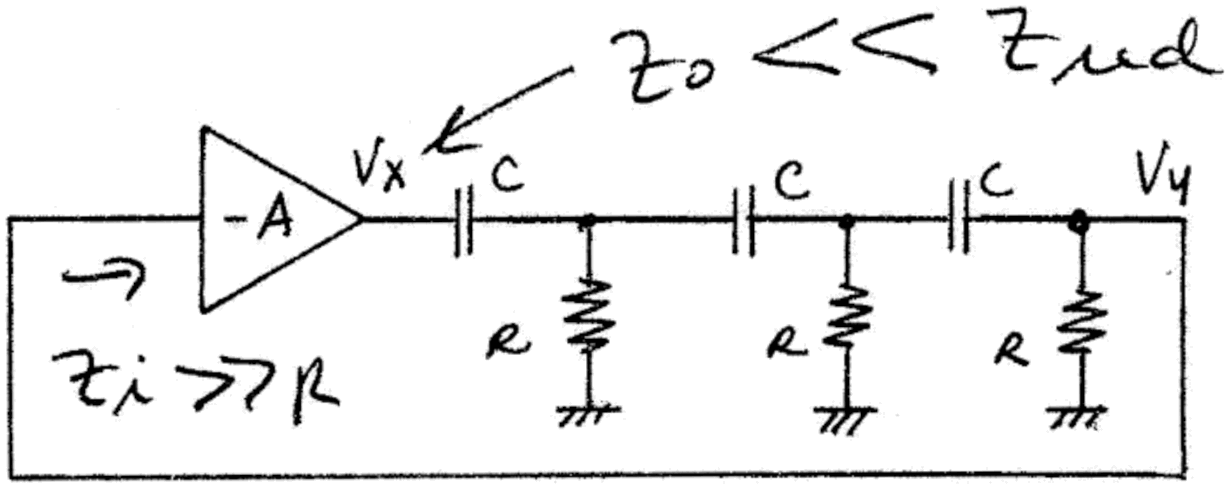
\includegraphics[width=0.8\linewidth]{_fig/osc_desplazamiento-de-fase-1opamp.png}
	\caption{Oscilador Desplazamiento de Fase con un solo amplificador}
	\label{fig:osc_desplazamiento-de-fase-1opamp}
\end{figure}

El amplificador simbolizado en la figura puede representar un operacional, un transistor o FET. En este caso el efecto de la red $\beta$ proporciona una función de transferencia total:

\[
\beta = \frac{V_y}{V_x} = \frac{1}{\left( 1-\frac{5}{\omega RC} - j \left( \frac{6}{\omega RC} - \frac{1}{\left( \omega RC \right)^3} \right) \right)}
\]

Se obtiene un desfasaje de $180^\circ$ si se obliga la parte imaginaria a ser cero, que se consigue para $1/(\omega RC)^2 = 6$, de donde la frecuencia de oscilación viene dada por:

\[
f = \frac{1}{2\pi RC\sqrt{6}}
\]

A esa frecuencia, $\beta = 1/29$, es decir que se requiere $|A| \geq 29$.

Se muestran configuraciones: con FET en la Figura \ref{fig:osc_desplazamiento-de-fase_fet}, con transistores ver Figura \ref{fig:osc_desplazamiento-de-fase_transistor} y con amplificador operacional ver Figura \ref{fig:osc_desplazamiento-de-fase_opamp-limitador}.

\begin{figure}[h]
	\centering
	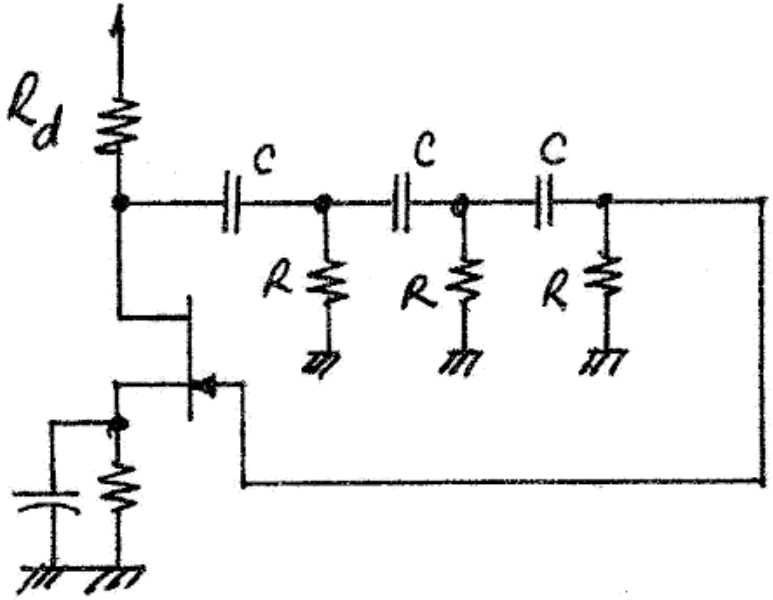
\includegraphics[width=0.8\linewidth]{_fig/osc_desplazamiento-de-fase_fet.png}
	\caption{Oscilador Desplazamiento de Fase, con FET}
	\label{fig:osc_desplazamiento-de-fase_fet}
\end{figure}

\begin{figure}[h]
	\centering
	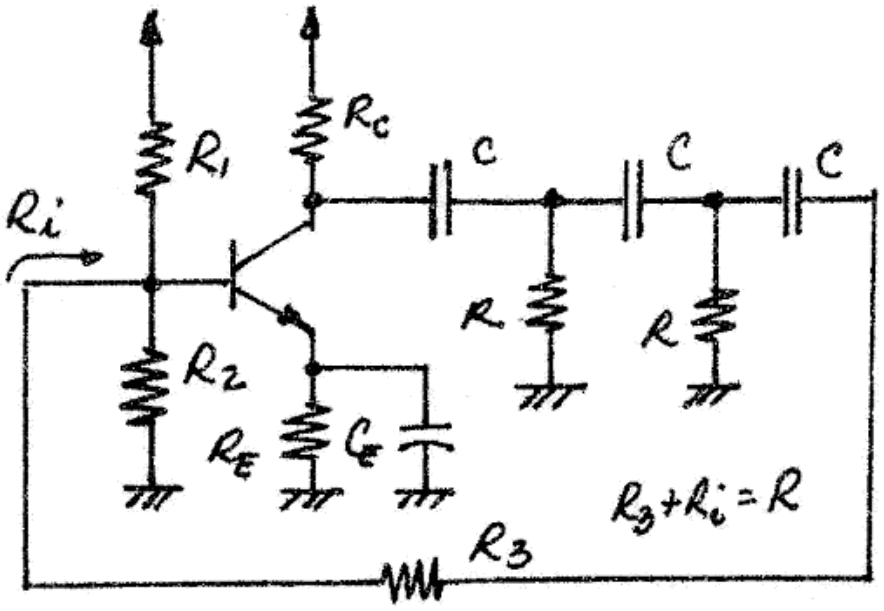
\includegraphics[width=0.8\linewidth]{_fig/osc_desplazamiento-de-fase_transistor.png}
	\caption{Oscilador Desplazamiento de Fase, con Transistor}
	\label{fig:osc_desplazamiento-de-fase_transistor}
\end{figure}

\begin{figure}[h]
	\centering
	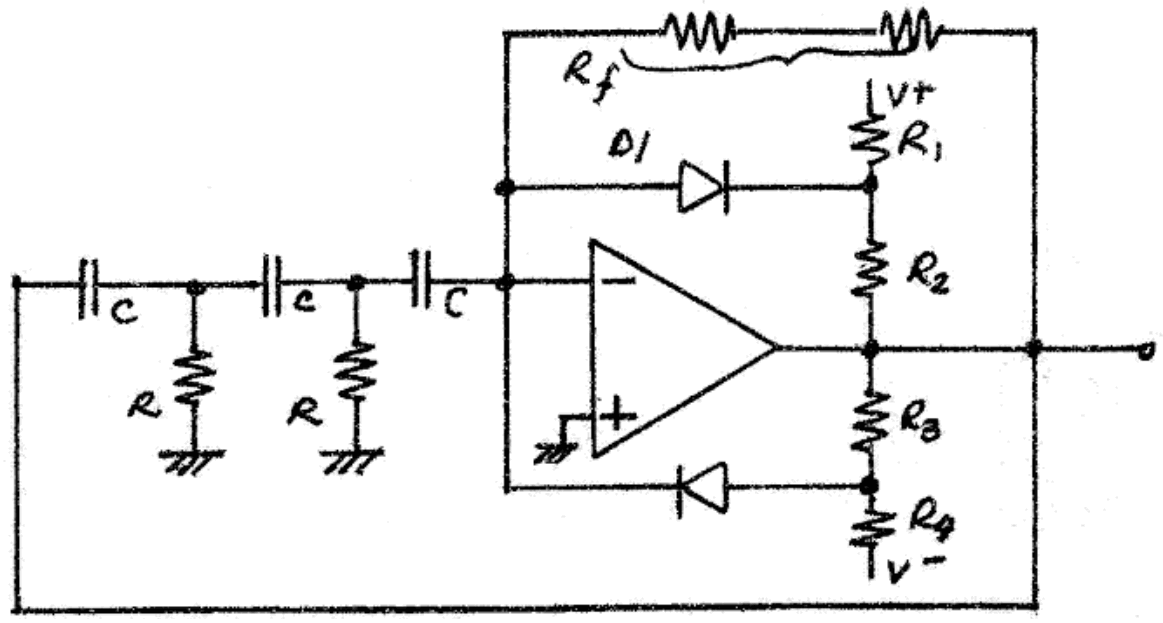
\includegraphics[width=0.8\linewidth]{_fig/osc_desplazamiento-de-fase_opamp-limitador.png}
	\caption{Oscilador Desplazamiento de Fase, con Op-Amp y Limitador}
	\label{fig:osc_desplazamiento-de-fase_opamp-limitador}
\end{figure}

Para que la configuración con FET oscile, una condición mínima a cumplir del FET es que $\mu = \frac{9n}{d}$ sea mayor que $29$.

El transistor en su configuración presenta una impedancia de entrada baja. Entonces se realimenta a la entrada con comparación de modo (corriente), y la $R$ de la última celda está formada por la suma de $R_3$ y la resistencia de entrada del transistor, $R_L$. Además se requiere $h_{fe} \geq 44,5$.

En la configuración con amplificador operacional, la red formada por $R_1$, $R_2$, $R_3$, $R_4$, $D_1$ y $D_2$ permite controlar la amplitud de la señal sinusoidal, si se consideran los demás elementos de la configuración como el oscilador básico; y se abre el lazo para determinar la ganancia del lazo, se obtiene:

\[
-A\beta = \frac{\omega^2 C^2 R R_f}{4+j(3\omega CR - \frac{1}{\omega CR})}
\]

La frecuencia de oscilación se encuentra obligando la parte imaginaria de esta expresión a ser cero, de donde

\[
\omega = \frac{1}{RC\sqrt{3}}
\]

A esa frecuencia requerimos que $-A\beta = 1$, por lo tanto

$\frac{\omega^2 C^2 R^2 R_f}{4R} = 1$, o $\frac{R_f}{R} = 12$, o $R_f = 12R$.

La relación $\frac{V^+ R_2}{R_1 + R_2}$ determina la amplitud máxima de la señal.

\subsection{Osciladores resonantes (Hartley-Colpitts)} %p212

El esquema de este tipo de oscilador se muestra en la Figura \ref{fig:osc_hartley-colpitts_esquema}; en la Figura \ref{fig:osc_hartley-colpitts_modelo} se ha reemplazado el amplificador por un modelo sencillo que tiene $R_s$ infinito, $A_v$ finito y $R_g$ finito. De este circuito se obtiene:

\[
-A\beta = \frac{-A_v Z_1 Z_2}{R_o(Z_1+Z_2+Z_3) + Z_2(Z_1+Z_2)}
\]

\begin{figure}[h]
	\centering
	\subfloat[Esquema General]
	{
		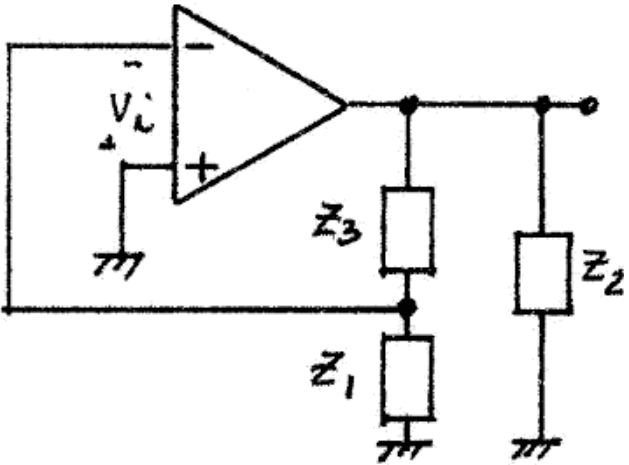
\includegraphics[width=0.4\linewidth]{_fig/osc_hartley-colpitts_esquema.png}
		\label{fig:osc_hartley-colpitts_esquema}
	}
	\subfloat[Modelo]
	{
		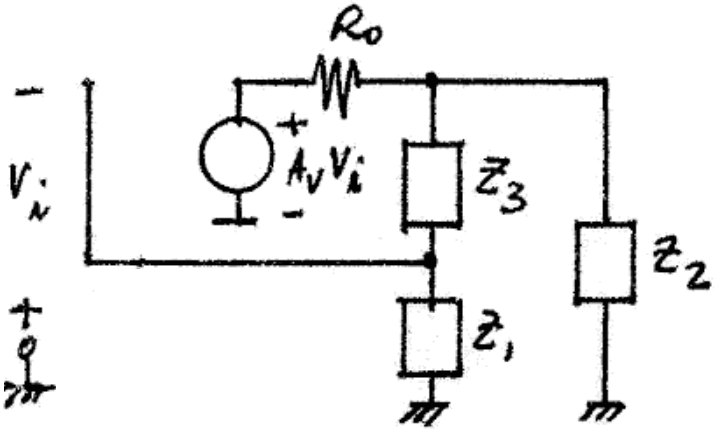
\includegraphics[width=0.4\linewidth]{_fig/osc_hartley-colpitts_modelo.png}
		\label{fig:osc_hartley-colpitts_modelo}
	}
	\caption{Oscilador de Tipo General}
	\label{fig:osc_hartley-colpitts}
\end{figure}

Si consideramos las $Z$ como impedancias reactivas, entonces $Z_1 = jX_1$, $Z_2 = jX_2$, $Z_3 = jX_3$, la expresión anterior se convierte en:

\[
-A\beta = \frac{A_v X_1 X_2}{j R_o(X_1 + X_2 + X_3) - X_2(X_1 + X_3)}
\]

Para que $-A\beta$ sea real, la parte imaginaria de esta expresión tiene que ser cero, de donde:

\[
X_1 + X_2 + X_3 = 0
\]

es decir, que la frecuencia de resonancia depende de la combinación serie de $X_1$, $X_2$, $X_3$. Cumplida esta condición entonces:

\[
- A \beta = \frac{A_v X_1 X_2}{-X_2 (X_1 + X_3) } = - \frac{A_V X_1}{X_1 + X_3}
\]

combinando ecuaciones se obtiene:

\[
- A \beta = \frac{A_v X_1}{X_2}
\]

de aquí podemos concluir que como $- A \beta$ tiene que ser positiva, entonces $X_1$ y $X_2$ tiene que ser del mismo signo, y por lo tanto $X_3$ del signo opuesto.

Si $X_1$ y $X_2$ son $C's$ y $X_3 = L$ el circuito es un oscilador Colpitts. Si $X_1$ y $X_2$ son $L's$ el circuito es un oscilador Hartley. Configuraciones prácticas de estos osciladores se muestran en la Figura \ref{fig:osc_hartley-colpitts_sch}.

\begin{figure}[h]
	\centering
	\subfloat[Colpitts]
	{
		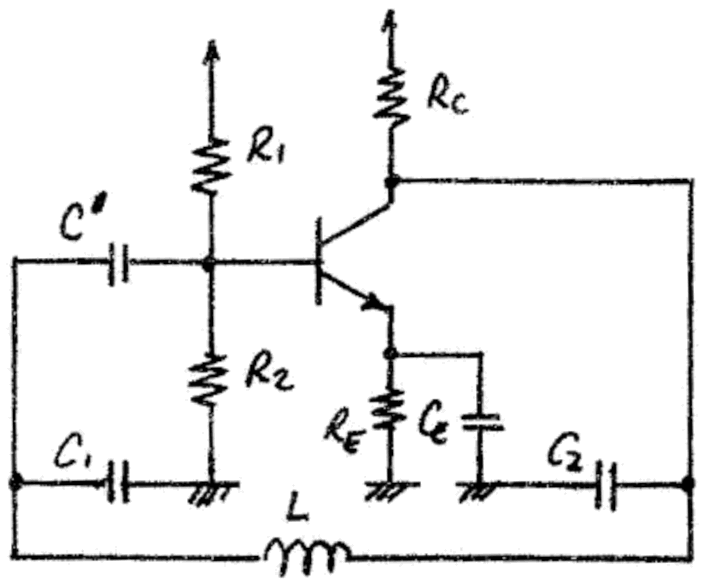
\includegraphics[width=0.4\linewidth]{_fig/osc_colpitts.png}
		\label{fig:osc_colpitts}
	}
	\subfloat[Hartley]
	{
		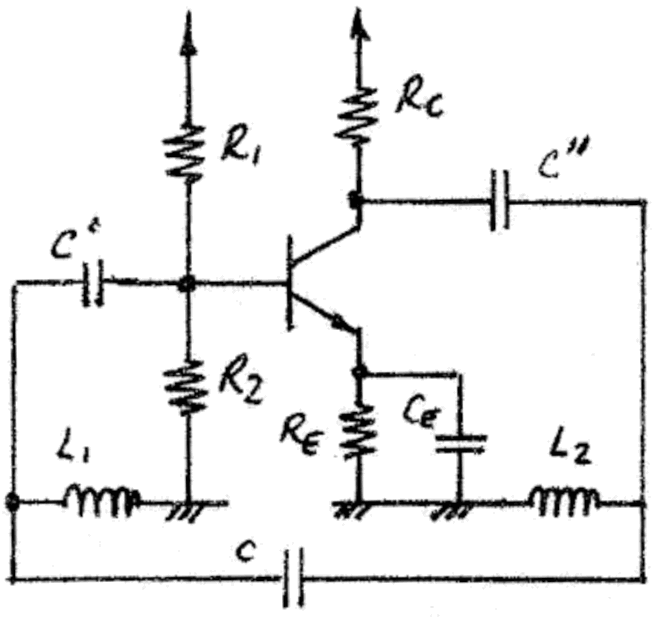
\includegraphics[width=0.4\linewidth]{_fig/osc_hartley.png}
		\label{fig:osc_hartley}
	}
	\caption{Oscilador de Tipo General}
	\label{fig:osc_hartley-colpitts_sch}
\end{figure}

\subsection{Oscilador puente de Wien} %p213

Este tipo de oscilador se muestra en la Figura \ref{fig:osc_puente-de-wien}.

\begin{figure}[h]
	\centering
	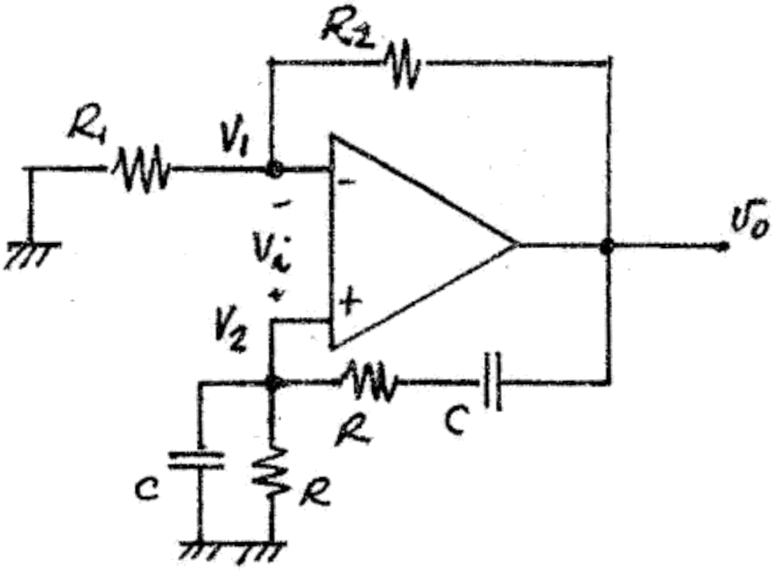
\includegraphics[width=0.8\linewidth]{_fig/osc_puente-de-wien.png}
	\caption{Oscilador Puente de Wien}
	\label{fig:osc_puente-de-wien}
\end{figure}

La rama de retroalimentación a la entrada negativa establece una ganancia de $1 + \frac{R_2}{R}$ (positiva). La red de retroalimentación a la entrada positiva tiene que presentar un desfasaje de $0^\circ$ para cumplir con un desfasaje total de ganancia de lazo, $-A\beta$, de $0^\circ$. La rama RC serie contribuye inicialmente en $f = 0$ con $+90^\circ$ y esta disminuye con $f$ hasta $0^\circ$, mientras la rama RC paralelo contribuye inicialmente en $f = 0$ con $0^\circ$, y esta disminuye con $f$ hasta $-90^\circ$. De modo que la combinación arranca con un desfasaje de $+90^\circ$ para terminar en $-90^\circ$. Cuando pasa por $0^\circ$ se obtiene la frecuencia de oscilación. A esa frecuencia se determina la atenuación de estas dos redes RC. Las resistencias $R_1$ y $R_2$ junto con el amplificador tendrán que compensar esta atenuación.

Analíticamente tenemos la función de transferencia de la red de retroalimentación:

\[
\frac{V_2}{V_0} = \frac{1/(sC) \parallel R}{1/(sC) \parallel R + R + 1/(sC)} = \frac{R}{R^2(1 + R s C)(R + 1/(sC))}
\]

\[
\frac{V_2}{V_0} = \frac{1}{1 + (1 + R s C)(1/(R s C))}
\]

La función de la fase viene dada por:

\[
\varphi = -\tan^{-1} \left( \frac{\omega R C - \frac{1}{\omega R C}}{3} \right)
\]

que será igual a $0$ cuando $\omega = \frac{1}{RC}$.

Reemplazando este valor de frecuencia en la función de transferencia anterior se obtiene:

\[
\frac{V_2}{V_0} = \frac{1}{1 + (1 + j)(1 - j)} = \frac{1}{3}
\]

De modo que se requiere $1 + \frac{R_2}{R_1} = 3$ o $R_2 = 2R_1$.

Un oscilador de Wien con estabilizador de amplitud se muestra en la Figura \ref{fig:osc_puente-de-wien_con-estabilizador}.

\begin{figure}[h]
	\centering
	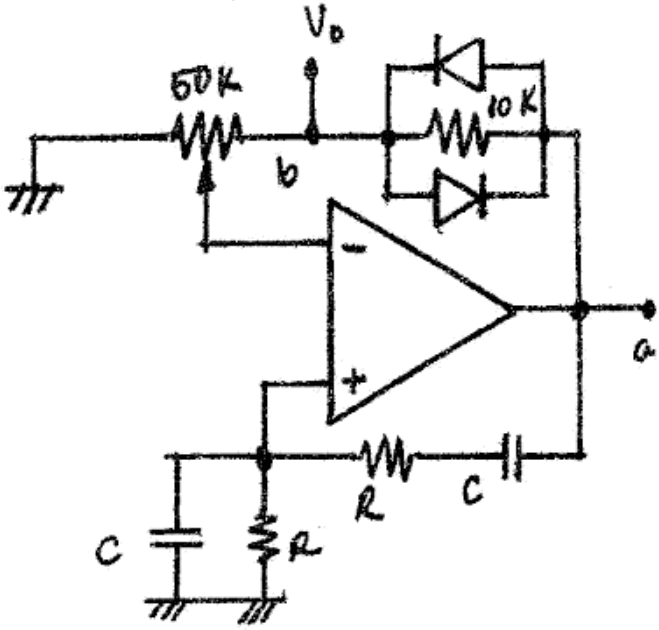
\includegraphics[width=0.8\linewidth]{_fig/osc_puente-de-wien_con-estabilizador.png}
	\caption{Oscilador Puente de Wien con estabilizador de amplitud}
	\label{fig:osc_puente-de-wien_con-estabilizador}
\end{figure}

El circuito de la figura tiene incorporado un mecanismo de variación de parámetro para el control de la amplitud.

El potenciómetro $P$ se ajusta hasta que comienzan a crecer las oscilaciones. Llegará el momento en que los diodos empiezan a conducir, reduciendo así la resistencia efectiva entre a y b, es decir, la ganancia de la configuración. El equilibrio se alcanzará cuando la amplitud de salida hace que la ganancia de lazo sea exactamente la unidad. La amplitud de salida puede ajustarse con $P$. La salida en $b$ tendrá menos distorsión que la de $a$; sin embargo, ésta es una salida de alta impedancia que requerirá una etapa amplificadora (buffer) para poder ser utilizada.

\subsection{Oscilador de cuadratura} %p215

Se muestra en la Figura \ref{fig:osc_oscilador-cuadratura}.

\begin{figure}[h]
	\centering
	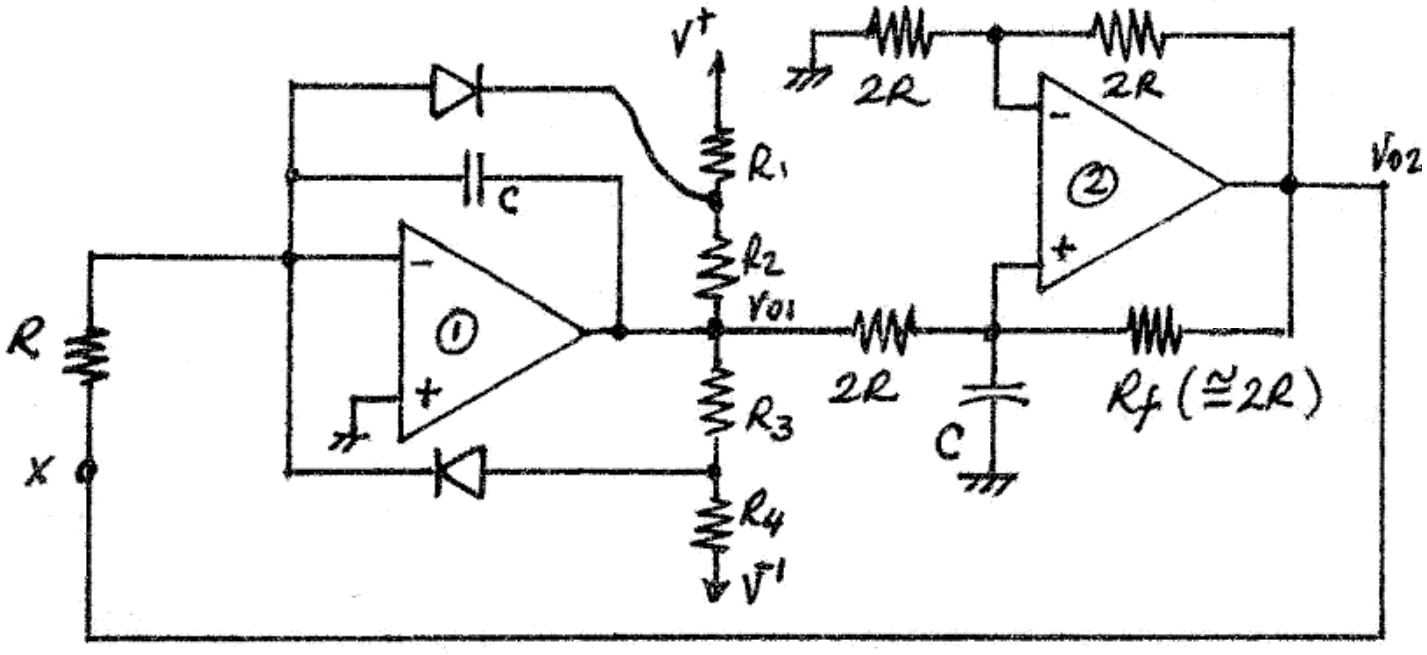
\includegraphics[width=0.8\linewidth]{_fig/osc_oscilador-cuadratura.png}
	\caption{Oscilador de Cuadratura}
	\label{fig:osc_oscilador-cuadratura}
\end{figure}

El amplificador $1$ está conectado como un integrador de ganancia negativa, y el $2$ como un integrador de ganancia positiva.

Si se encuentra la ganancia del lazo... por ejemplo, abriendo el lazo en $X$ se encuentra:

\[
-AB = \frac{V_2}{V_x} = -\frac{1}{s^2 C^2 R^2}
\]

de donde el lazo oscilará a la frecuencia:

\[
\omega = \frac{1}{RC}
\]

El circuito suministrará dos salidas senoidales, en $V_{O1}$ y $V_{O2}$, con un desfase de $90^\circ$ entre ellas.

\subsection{Oscilador de filtro activo sintorizado} %p216

El esquema se muestra en la Figura \ref{fig:osc_filtro-activo-sintonizado_esquema}.

\begin{figure}[h]
	\centering
	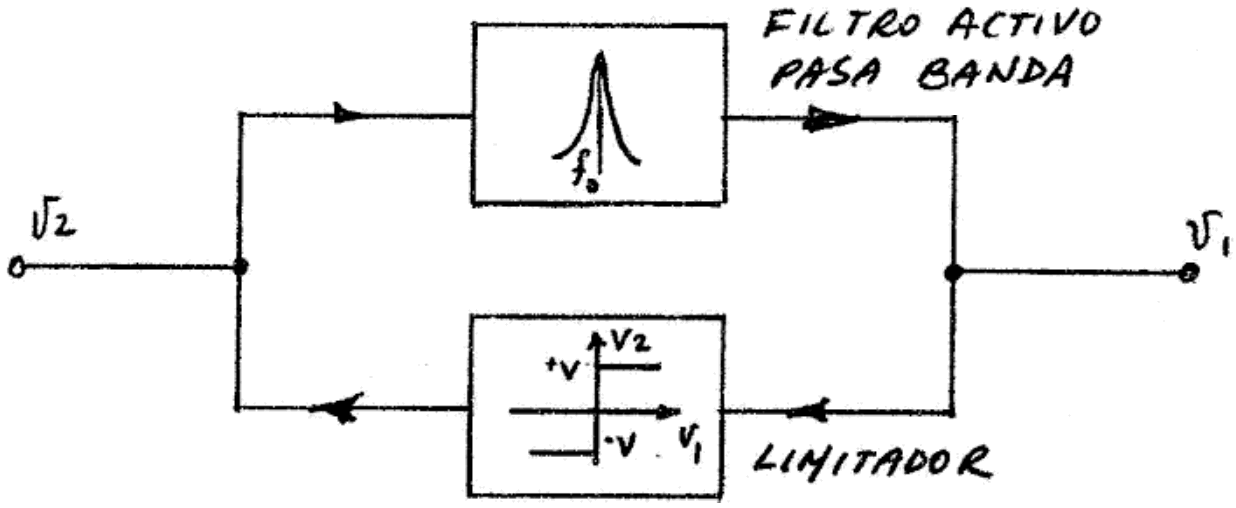
\includegraphics[width=0.8\linewidth]{_fig/osc_filtro-activo-sintonizado_esquema.png}
	\caption{Oscilador de Filtro Activo Sintonizado}
	\label{fig:osc_filtro-activo-sintonizado_esquema}
\end{figure}

Se tiene un filtro activo pasa banda de $Q$ elevado conectado en un lazo de retroalimentación positiva con un limitador. Suponer que las oscilaciones ya han arrancado. La salida del filtro activo será una onda senoidal de frecuencia $f_0$. Esta señal sirve de entrada al limitador, que generará una onda cuadrada de salida de frecuencia $f_0$. Esta a su vez sirve de entrada al filtro que eliminará las armónicas superiores para así producir una onda senoidal. La pureza de la onda senoidal será función de la calidad (factor $Q$) del filtro activo. Tiene la ventaja de permitir el control independiente de la amplitud y de la frecuencia. En la Figura \ref{fig:osc_filtro-activo-sintonizado_circuito} una configuración práctica.	

\begin{figure}[h]
	\centering
	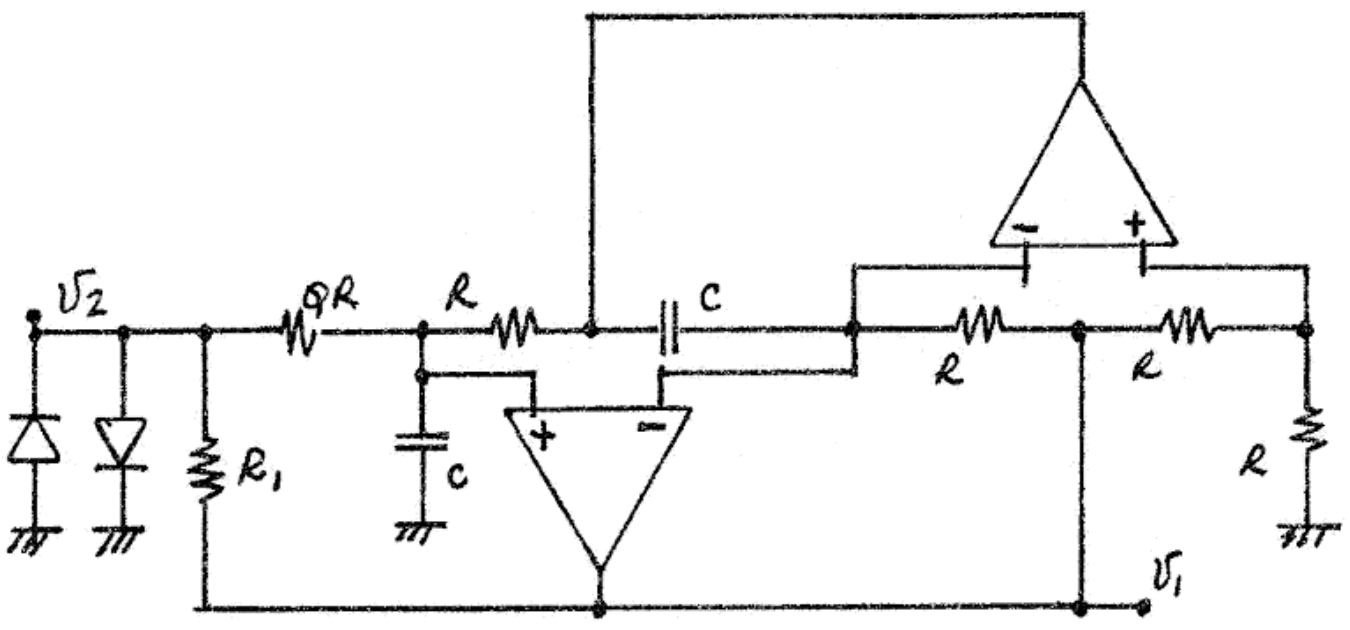
\includegraphics[width=0.8\linewidth]{_fig/osc_filtro-activo-sintonizado_circuito.png}
	\caption{Oscilador de Filtro Activo Sintonizado}
	\label{fig:osc_filtro-activo-sintonizado_circuito}
\end{figure}

\section{Problemario} %p219

- pendiente en apuntes -